\documentclass[12pt,letterpaper ,oneside , openright]{book}
\usepackage{thesis}
%para desarrollo
	%\usepackage{showframe}
	%\includeonly{usingTheLibrary_chapter,usingthelibrary/compresibilityFactor,usingthelibrary/fugacity,usingthelibrary/volume,apendixEquations,usingthelibrary/parameters}     
	%\includeonly{usingthelibrary/alphaOptim,usingthelibrary/binaryOptim, apendixEquations,alpha/alphas}
	%\includeonly{usingthelibrary/units}
	%\includeonly{webpage_chapter}
	%\includeonly{libraryExtension_chapter}
	%\includeonly{githubAppendix}
	%\includeonly{apendixEquations}
%--               
\begin{document}      
	\begin{titlepage}
	\begin{minipage}[c][9in][s]{1in}
	\centering
	
\includegraphics[width=1in]{Escudo-UNAM}\\[10pt]
	\hskip 2pt\vrule width 2pt height 6.7in
	\hskip 1mm\vrule width 1pt height 6.7in\\[10pt]
	
\includegraphics[width=1in]{images/FQ.jpg}
	\end{minipage}\hskip 10pt
	\begin{minipage}[c][\textheight][s]{5.125in}
	\centering
	{\textsc{ \large{Universidad Nacional Autónoma De México}}}
	\vspace{3mm}\hrule height2pt
	\vspace{1mm}\hrule height1pt
	\vspace{3mm}
	\textsc{Facultad De Química}\\[3cm]
	\textsc{\Large Desarrollo de una librería en java para el cálculo de propiedades de sustancias con ecuaciones de estado cúbicas}\\[3cm]
	\makebox[8cm][s]{\Huge T E S I S}\\[8pt]
	\textsc{ que para obtener el título de }\\[3pt]
	\textsc{ Ingeniero Químico}\\[1cm]
	\textsc{ presenta: }\\[0.3cm]
	\textsc{ Hugo Redon Rivera }\\[0.5cm]
	\vfill
	{\scshape {México, D.F.} \hfill{2014} }	
	\end{minipage}
\end{titlepage}
\newpage
\begin{minipage}[c][\textheight][s]{5.125in}
JURADO ASIGNADO:\\[0.5cm]

PRESIDENTE:		Profesor:\\
VOCAL: 		Profesor:\\
SECRETARIO:		Profesor:\\
1er.  SUPLENTE: 	Profesor:\\
2° SUPLENTE:		Profesor:\\[0.5cm]

\begin{center}
	SITIO DONDE SE DESARROLLÓ EL TEMA:\\
	\textsc{Facultad de Química}\\[3cm]


	\rule{6cm}{1pt}\\
	\textsc{asesor del tema: Dr. Enrique Rodolfo Bazúa Rueda.} \\[3cm]


	\rule{6cm}{1pt}\\
	\textsc{SUSTENTANTE:Hugo Redon Rivera.} 
\end{center}
\end{minipage}
%Portada -Hecho
	\tableofcontents	
	\listoffigures
	\listoftables
	\chapter{Objetivos}

\begin{itemize}
	\item Desarrollar una biblioteca escrita en el lenguaje de java para realizar:
	\begin{itemize}
		\item El cálculo de propiedades de sustancias puras y mezclas con ecuaciones de estado cúbicas.
		\item Cálculos de equilibrio Líquido-Vapor.
		\item La estimación de parámetros de expresiones de $\alpha$ para el cálculo de la constante $a$ de la ecuación de estado cúbica.
		\item La estimación de parámetros binarios de las reglas de mezclado para el cálculo de las constantes $a$ y $b$ para mezclas.
	\end{itemize}
	\item La biblioteca a desarrollar deberá ser versátil, robusta, simple de usar y fácilmente expandible.
	\item Desarrollar una interfaz de usuario que exponga las funciones de la librería.
	\item Proponer un medio de difusión de la librería, que sea capaz de involucrar a cualquier persona interesada en modificar y extender la librería.
\end{itemize}

\chapter{Introducción}

	Esta tesis trata sobre el uso de métodos computacionales para el cálculo de propiedades volumétricas y puntos de equilibrio Líquido-Vapor con ecuaciones de estado cúbicas. 

	Como resultado se ha escrito una biblioteca de clases en java denominada \textbf{Materia}.

	El diseño de la biblioteca en conjunto con las herramientas que se describen en la sección \ref{chap:tools} hacen de este trabajo una plataforma para el desarrollo de aplicaciones de simulación y modelado de procesos quimicos industriales.

	El presente trabajo propone un procedimiento para el desarrollo de futuras aplicaciones. Para lo cual se ha dotado de ciertas características a la biblioteca \textbf{Materia} asegurando el funcionamiento del proceso propuesto.

	La biblioteca \textbf{Materia} se ha escrito para que su utilizacióń sea sencilla y no se requieran grandes conocimientos sobre programación. El capítulo \ref{chap:libraryUse} muestra como utilizar la estructura de clases para realizar los cálculos de propiedades y de equilibrio, mostrando pequeños fragmentos de código.

	El capítulo \ref{chap:libraryExtension} muestra como extender la biblioteca de clases, guía en el proceso de creación de nuevas reglas de mezclado, expresiones de $\alpha$, etc. Este capítulo supone un conocimiento mas avanzado en temas de programación orientada a objetos.

	Se ha creado una página de internet para permitir el uso de la librería \textbf{Materia} a través de una interfaz de usuario, el capítulo \ref{chap:webPage} documenta las funciones de la página. También es posible extender las funciones de la página de internet, sin embargo son necesarios conocimientos que estan fuera del alcance de esta tesis. El apéndice \ref{chap:webTools} describe las tecnologías utilizadas para la creación de la página de internet, y una breve descripción de su estructura.
	%\marginpar{Explicación de las ecuaciones y cálculos que se realizan,Versatilidad del programa,Descripción de la estructura de la tesis,Alcance de la aplicación}
	%Objetivos -Hecho
	\chapter{Herramientas}
	\section{Java}
		Un lenguaje simple, orientado a objetos, distribuido, interpretado, robusto, de arquitectura neutral, portátil, de alto rendimiento, seguro, multiproceso y dinámico.\cite{java} 

		Definición dada por James Gosling \footnote{Considerado creador del lenguaje Java}  en la fecha de su primer publicación (1995). 

		\begin{description}
		\item{Simple:} Una de las razones mas importantes por las que se decidió programar la librería en este lenguaje es que java evita al programador la necesidad de realizar tareas de índole técnico sobre la computadora, como por ejemplo el almacenamiento de los datos en la memoria. Esto permite al programador concentrarse en el area de estudio deseada.

		\item{Orientado a objetos:}
		Sin duda la perspectiva orientada a objetos de java es otro gran atractivo para las ciencias e ingenierías. La división y clasificación de las ramas de estudio permiten concentrarnos en todos y cada uno de los aspectos importantes sobre el tema. De igual manera la division de un programa en objetos nos permite concentrarnos en los aspectos y actividades importantes. Tómese como ejemplo la clasificación de la materia en homogénea y heterogénea, el aspecto importante en esta clasificación es la presencia de uno o más estados de agregación en el sistema, se puede pensar así en un cálculo de equilibrio Líquido-Vapor para un sistema heterogéneo, pero no para un sistema homogéneo.

		\item{Distribuido:}
		Java es una de las principales herramientas para el desarrollo web, un invento solo comparable con la imprenta. Su importancia radica en su capacidad de difusión masiva. La creación de un servicio o cualquier producto es tan importante como su difusión. En conjunto con la librería de funciones se ha creado un sitio web donde se exponen algunas de las funciones mas importantes de la librería.

		\item{De arquitectura neutra:}
		Java es multiplataforma, lo cual significa que puede ser ejecutado en la gran mayoría de los sistemas operativos existentes en el mercado actual.

		\end{description}

	\section{JUnit}

		Esta librería de funciones \footnote{Librería de funciones es una traducción de ``java class library'', que es el nombre del tipo de proyecto del presente trabajo. Una mejor definicion sería una ``Estructura de objetos''} ha sido creada con la idea de expandirse y ser escrita por cualquier persona interesada en ello.Es muy importante mantener una evidencia del funcionamiento de la librería. El uso de la tecnología JUnit es una forma para asegurar que los cambios introducidos al programa no han afectado el funcionamiento esperado de la libreria.

		Al momento de escribir este trabajo la librería cuenta con mas de 100 pruebas que definen un funcionamiento.

		\subsection{Desarrollo basado en pruebas}
	\section{Git}

		Git es un sistema de gestión y distribución de código fuente. Permite llevar un registro de los cambios realizados, utilizar las diferentes versiones, y compartir los cambios entre usuarios.

	\section{GitHub}

		GitHub es un servicio de depósitos de repositorios Git. Es un sitio donde se puede guardar el código fuente, es muy fácil contribuir al proyecto y compartir los cambios propuestos, es accesible a todo el público.

	\section{Maven}

		Maven es una herramienta de construcción de código, una de sus grandes ventajas es que puede descargar de manera segura versiones compiladas de proyectos con unas pocas lineas de código. Mas adelante se detallara el proceso de uso.

	\section{Netbeans}
		NetBeans es un entorno de desarrollo integrado para el desarrollo principalmente con Java, pero también con otros lenguajes, en particular, PHP, C / C++, y HTML5. También es una estructura la plataforma de aplicaciones para aplicaciones de escritorio Java y otros.
	

	\section{Openshift}
		OpenShift es una plataforma de programación en la nube orientada a servicios de Red Hat. Una versión para la nube privada se llama OpenShift Enterprise. El software que ejecuta el servicio se encuentra bajo el nombre "OpenShift Origin" de código abierto y está disponible en GitHub.

	\section{Wildfly}
		WildFly, anteriormente conocido como "JavaBeans Open Source Software Application Server" es un servidor de aplicaciones que implementa la plataforma Java, Enterprise Edition. JBoss está escrito en Java y como tal es multiplataforma: utilizable en cualquier sistema operativo que soporte Java

	\section{GNU GENERAL PUBLIC LICENSE Version 2}

		"GNU GENERAL PUBLIC LICENSE" es una licencia libre, sin derechos para software y otro tipo de obras. Pretende garantizar la libertad de compartir y modificar todas las versiones de un programa - para asegurarse de que sigue siendo software libre para todos sus usuarios.
		
	\section{Idioma}

		Existen dos razones por la que se ha elegido el idioma inglés para expresar las funciones de la librería. La primer razon y las mas importante, es que java ha sido escrito en inglés y por lo tanto las estructuras de control y palabras reservadas. Pongamos como ejemplo el siguiente fragmento de código.

\begin{lstlisting}
public boolean isItADog(Pet pet){
	if ( pet.getSpeciesName().equals("Canis lupus familiaris")) {
		return true;
	}else{
		return false;
	}
}
\end{lstlisting}

	El fragmento de código pretende conocer si el nombre de la especie de la mascota es el nombre científico "Canis lupus familiaris", si es asi devuelve verdadero, de lo contrario falso. Veamos ahora la versión en español para el mismo fragmento de código.

\begin{lstlisting}
public boolean esUnPerro(Mascota mascota){
	if ( mascota.getNombreDeLaEspecie().equals("Canis lupus familiaris")){
		return true;
	}else{
		return false;
	}
}
\end{lstlisting}

	En inglés, el order de las palabras denota la diferencia entre una pregunta y una afirmación, de modo que el nombre del método en inglés claramete indica la pregunta "Is it a Dog?" cuando en español la diferencia entre la pregunta y la afirmación debe ser escrita con un signo de interrogación "¿Es un perro?" sin ellos el nombre del metodo puede parecer la afirmación "Es un perro!".

	También puede notarse el nombre del método "getNombreDeLaEspecie", el prefijo "get" es una convención en java que significa recuperar, se usa para obtener el valor de la variable que continúe al prefijo, sin el prefijo estaríamos restringiendo la funcionalidad de la librería.

	Puede apreciarse que la lectura de la línea en ingles es fluida.No existe la necesidad de realizar traducciones. Aunque parezca trivial en este ejemplo, en porciones mas grandes de código la diferencia es bastante notable.

	Quiero hacer notar que en ningún momento se intenta hacer una comparación sobre los idiomas, sino señalar el beneficio de la fluidez que se obtiene al no mezclarlos.

	%Sobre java y herramientas -Hecho
	\chapter{Instalación}

  Para instalar la biblioteca \textbf{Materia} es necesario saber que tipo de trabajo se desea realizar con ella:
  \begin{itemize}
    \item Crear una aplicación que emplea las funciones ya definidas en la biblioteca.
    \item Crear una nueva funcionalidad de la biblioteca.
  \end{itemize}

  Por ejemplo si se desea escribir una aplicación que realize diagramas de presión contra volumen molar usando ecuaciones de estado cúbicas, solo será necesario instalar la forma compilada según la sección \ref{sec:compiledinstall}. Ya que las funciones para calcular la presión y el volumen molar con ecuaciones de estado cúbicas existen en la biblioteca , no será necesario modificar el código fuente, por lo tanto no es necesaria la instalación del código fuente. En cambio si se desea utilizar ecuaciones viriales para realizar los diagramas de presión, se deberán realizar las dos instalaciones descritas en este capítulo, ya que las ecuaciones viriales no forman parte del alance de esta tesis, la librería debera ser extendida para incluir dichas ecuaciones, una vez hecha la extensión al código fuente , la versión compilada puede ser empleada para realizar la aplicación que realice los diagramas.


  \section{Para uso de la librería (compilado)}\label{sec:compiledinstall}

      Existen dos formas de utilizar la librería Materia en una aplicación java:
    Descargar el archivo .jar y agregarlo al folder /lib de la aplicación ó desde maven utilizando el archivo pom.xml.

    La librería existe como un archivo .jar, se puede descargar desde la página creada para su difusión \url{ingenieria-eqpro.rhcloud.com}, o automáticamente desde los servidores de sonatype haciendo uso de maven.

    Si se realiza la instalación manual la ubicación de la librería depende de la estructura del proyecto, por ejemplo para una aplicación web los archivos jar deberán ser agregados en el folder dentro del proyecto src/main/webapp/WEB-INF/lib.

    Utilizando maven solo deberán agregarse las siguientes lineas de código al archivo pom.xml.

    \begin{lstlisting}[language=XML,morekeywords={repositories,
    repository,id,name,url,groupId,artifactId,dependencies,dependency}]
<dependencies>
  <dependency>
   <groupId>com.github.hugoredon</groupId>
   <artifactId>materia</artifactId>
   <version>1</version>
  </dependency>
</dependencies>
\end{lstlisting}

    En el apéndice \ref{sec:manualInstall} se ejemplifica la instalación manual y en el apéndice \ref{sec:mavenInstall} se muestra la instalación vía maven, para una aplicación de escritorio.


  \section{Para extender o modificar la librería (código fuente)}

    El código fuente de la librería se expone de manera pública en la página \url{https://github.com/HugoRedon/Materia}, bajo la licencia GNU GENERAL PUBLIC LICENSE Version 2.
  
    Para poder participar en el proyecto será necesario obtener de manera gratuita una cuenta en github, realizar una copia o clon \footnote{En github a una copia de un proyecto se conoce como ``Fork''} de la librería  a la nueva cuenta, copiar el código fuente a la computadora haciendo uso de git,realizar los cambios y agregarlos a la cuenta en GitHub  \footnote{El procedimiento hace uso de los comandos `git clone', `git commit' y `git push', que son explicados con mas detalle en el apéndice \ref{chapgithub}} ,finalmente hacer una petición para integrar los cambios a la librería original ``Pull request'', y si los cambios son aceptados, se habrá logrado la participación al proyecto. El proceso se detalla en el apéndice \ref{chap:github}.



%Sobre la instalación Hecho
	\chapter{Uso de la librería}\label{chap:libraryUse}
	
	Dada la extensión de la librería, no resulta posible ni deseable mostrar el código fuente completo\footnote{El código completo puede ser consultado y descargado desde la página \url{https://github.com/HugoRedon/Materia}. El apéndice \ref{chap:github} guía al lector en el procedimiento de modificación o extensión del código fuente.}, en este capítulo se presentan pequeños fragmentos de código que muestran la forma de utilizar la librería y su estructura.
		
	La clase `Cubic' realiza cálculos de presión, fugacidad, factor de compresibilidad y adimensionamiento de los parámetros $a$ y $b$, pero no calcula los parámetros $a$ y $b$.Para calcular los parámetos $a$ y $b$ existen las clases `Substance' y `Mixture' que definen el cálculo de los parámetros para un compuesto puro o para una mezcla respectivamente. 

	Las clases `Substance' y `Mixture' tienen en común los métodos `calculate\_a\_cubicParameter', `calculate\_b\_cubicParameter', ademas de otros que se condensan en la clase `Homogeneous'.La clase `Homogeneous' utiliza los cálculos de los parámetros de la ecuación cúbica y la clase cúbic para finalmente realizar el cálculo de la fugacidad, presión ,factor compresibilidad, entalpía, entropía y energía libre de Gibbs.

	La clase `Homogeneous' no realiza cálculos de equlibrio, ya que la clase representa una sola fase. Para realizar cálculos de equilibrio existe la clase `Heterogeneous' que contiene dos fases una líquida y una vapor. A través de los cálculos de fugacidad de cada fase y empleando un algoritmo numérico se pueden realizar los cálculos de equilibrio Líquid-Vapor.


	Las secciones del capítulo:
	\begin{itemize}
		\item{Sección} \ref{sec:units} Se definen las unidades que emplearan durante todo el capítulo.
		\item{Sección} \ref{sec:cubic}  La clase `Cubic' realiza cálculos de presión, fugacidad, factor de compresibilidad y volumen molar.
		\item{Sección} \ref{sec:compounds} La clase `Compound' para definir y utilizar las propiedades del compuesto puro dentro de la librería.
		\item {Sección} \ref{sec:parameters} La clase `Homogeneous' y sus implementaciones `Substance' y `Mixture' para calcular los parámetros de la ecuación cúbica.
		\item {Sección} \ref{sec:homogeneous} La clase `Homogeneous' para realizar cálculos de entalpía, entropía y energía libre de Gibbs.
		\item {Sección} \ref{sec:heterogeneous} La clase `Heterogeneous' y sus implementaciónes `HeterogeneousSubstance' y `HeterogeneousMixutre' para realizar cálculos de equilibrio Líquido-Vapor.
	\end{itemize}
%hecho

		\section{Sistema de Unidades}\label{sec:units}

Las unidades que utiliza la librería se muestran en la tabla \ref{tab:units}.
Durante este escrito se utilizarán las mismas unidades, a menos que se indique lo contrario.


\begin{table}[!h]
	\centering
	\caption{Sistema de unidades empleado por la librería}\label{tab:units}
	\begin{tabular}{ |c| c|c|}
		\hline
			Propiedad & Unidad &\\
		\hline
			Presión & $Pa$ & Pascal\\
			Temperatura & $K$ & Kelvin\\
			Volumen molar & $\frac{m^3}{kg}$ & Metro cúbico sobre kilogramo\\

		\hline
	\end{tabular}
\end{table}%hecho
		\section{Ecuación de estado cúbica}\label{sec:cubic}

	La ecuación de estado cúbica representada por la clase `Cubic', permite realizar los cálculos de: 
	\begin{itemize}	\itemsep0ex
		\item Presión
		\item Factor de compresibilidad
		\item Volumen molar
		\item Fugacidad
	\end{itemize}

	Cualquier ecuación de estado cúbica se puede crear dentro de la librería \Materia usando los métodos `get' y `set' de la clase `Cubic', ver la sección \ref{subsec:cubicCreation}, pero para comodidad se han definido las ecuaciones de la tabla \ref{tab:cubics} para accederse a través de la clase `EquationsOfState'.

	\begin{table}[!h]
		\centering
		\caption{Ecuaciónes de estado cúbicas accesibles desde la clase `EquationsOfState'}\label{tab:cubics}
		\begin{tabular}{|c |c | c | c | c |}
			\hline
			Ecuación de estado  & $u$ & $w$ & $\Omega_a$&$\Omega_b$\\
			\hline
			Van Der Waals  & $0$ & $0$ & $0,421875$ & $0,125$\\
			\hline
			Peng robinson  & $2$ & $-1$ & $0.45723553$ & $0.077796074$\\
			\hline
			Redlich Kwong  & $1$ & $0$ & $0.42748023$ & $0.08664035$\\
			\hline
			TST  & $2.5$ & $-1.5$ &$ 0.470507$ & $0.0740740$\\
			\hline
		\end{tabular}		
	\end{table}

\subsection{Creación de una ecuación de estado cúbica}\label{subsec:cubicCreation}

	Existen dos formas de crear una ecuación cúbica dentro de la librería \Materia.

	La primera es a través del método contructor, que se accede con la palabra reservada  `new'. De esta manera los valores u y w de la ecuación de estado son iguales a 0 y se les puede asignar un valor diferente haciendo uso de los métods `get' y `set' como se muestra en el código \ref{lst:pengRobinsonCreation}.

	\begin{lstlisting}[label={lst:pengRobinsonCreation},caption=Creación de la ecuación de estado de Peng Robinson usando los metodos `Set' de los parametros u y w]
	Cubic pengRobinson = new Cubic();
	pengRobinson.setU(2);
	pengRobinson.setW(-1);
	pengRobinson.setOmega_a(0.45723553);
	pengRobinson.setOmega_b(0.077796074);
	\end{lstlisting}

	La segunda forma de crear una ecuación de estado es a través de la clase `EquationsOfState'. Para obtener una ecuación con los parámetros previamente establecidos, el fragmento de código \ref{lst:tstCreation} muestra el procedimiento.


	\begin{lstlisting}[label=lst:tstCreation,caption=Creación de la ecuación de estado de TST usando la clase `EquationsOfState']
	Cubic tst = EquationsOfState.twoSimTassone();
	\end{lstlisting}

\subsection{Cálculos con la ecuación cúbica}
	Ya que la clase `Cubic' no realiza los cálculos de sus parámetros estos deben ser proporcionados como argumento de los métodos.

	Los métodos de la clase `Cubic' raramente será necesario usarlos directamente, ya que es dificil obtener el cálculo de los parámetros $a$ y $b$, en cambio la clase `Homogeneous' define el cálculo de los parámetros y de las propiedades que a continuación se muestran.

	\subsubsection{Presión}
	El cálculo en el método `calculatePressure' se realiza según la ecuación \ref{eq:pressure} y se utiliza como se muestra en el código \ref{lst:cubicpressure}.
\begin{lstlisting}[label={lst:cubicpressure},caption={Cálculo de presión con una ecuación de estado cúbica, proporcionando como argumento la temperatura, el volumen y los parámetros $a$,$b$}]
	 double pressure =  cubic.calculatePressure(temperature, volume, a, b);
\end{lstlisting}
	\subsubsection{Factor de compresibilidad}

	Es necesario realizar la solución de la ecuación de estado cúbica, como se muestra en el apéndice \ref{sec:cubicsolution}, para conocer el factor de compresibilidad. La solución de la ecuación se realiza en el método `calculateCompresibilityFactor'.

	El método recibe los parámetros adimensionales A, B y la fase a la cual se desea calcular el factor de compresibilidad. La clase ``Cubic'' tiene los métodos necesarios para transformar los parámetros a y b a su forma adimensional A y B según las ecuaciones \ref{eq:AB}.

	El código \ref{lst:cubiccompresibility} muestra como usar el método.
\begin{lstlisting}[label={lst:cubiccompresibility},caption={Cálculo del factor de compresibilidad con una ecuación de estado cúbica, proporcionando como argumento los parámetros adimensionales $A$,$B$, y la fase a la cual se desea calcular el factor}]
	double z = cubic.calculateCompresibilityFactor(A,B,phase);
\end{lstlisting}
	\subsubsection{Volumen molar}

	La ecuación \ref{eq:volume} proporciona un método para calcular el volume molar a partir del factor de compresibilidad. El código \ref{lst:cubicvolume} muestra el método.
\begin{lstlisting}[label={lst:cubicvolume},caption={Cálculo del volumen molar usando una ecuación de estado cúbica, el método recibe los parámetros de temperatura, presión y factor acéntrico}]
	double volume = calculateVolume(temperature, pressure, z);
\end{lstlisting}	
	\subsubsection{Fugacidad}
	La fugacidad se calcúla segun la ecuación \ref{eq:fugacity}.Para realizar el cálculo de la fugaciad es necesario conocer las derivadas de los parámetros con respecto a la cantidad de moles del componente i, es decir al componente para el cúal se desea realizar el cálculo de fugacidad. El cálculo de la derivada de los parámetros se realiza en las clases que hereden a `Homogeneous', por ejemplo las clases `Substance' y `Mixture'.
	El método se usa como se indica en el código \ref{lst:fugacity}.
\begin{lstlisting}[label={lst:fugacity},caption={Cálculo de fugacidad usando una ecuación de estad cúbica, el método recibe los parámetros de temperatura, presión ,los parámetros de la ecuación cúbica $a$ y $b$, las derivadas con respecto a la cantidad de moles $partial_a$, $partial_b$ y finalmente la fase a la que se desea el cálculo de la fugacidad.}]
	double fugacity = calculateFugacity(temperature, pressure,
										 a, b, parcial_a, parcial_b,phase);
\end{lstlisting}


%hecho
		\section{Compuestos}\label{sec:compounds}

La clase `Compound' permite definir las propiedades de un compuesto puro y utilizarlas dentro de la librería \Materia.

Propiedades como la temperatura crítica, presión crítica, factor acéntrico y los parámetros para las expresiones de \alfa pueden obtenerse de esta clase como se muestra en el código \ref{lst:compounds}.

\begin{lstlisting}[caption={Se muestra la creación de un objeto tipo `Compound' para definir y utilizar las propiedades del cyclohexano, haciendo uso de los métodos `get' y `set'.},label={lst:compounds}]
Compound compound = new Compound("Cyclohexane");
compound.setCriticalPressure(4073000);
compound.setCriticalTemperature(553.5);
compound.setAcentricFactor(0.211);
....
double acentricFactor = compound.getAcentricFactor();
double pc = compound.getCriticalPressure();
double tc = compound.getCriticalTemperature();
\end{lstlisting}






%hecho
		\section{Parámetros de la ecuación de estado cúbica}\label{sec:parameters}

El cálculo de los parámetros depende de la cantidad de compuestos presentes en el sistema.

\begin{itemize}
 \item Para los compuestos puros la clase `Substance' define el cálculo de los parámetros usando una expresión de $\alpha$ , los parámetros $\Omega_a$ y $\Omega_b$ de la ecuación de estado y las propiedades del compuesto puro.
 \item Para las mezclas, la clase `Mixture' define el cálculo de los parámetros usando una regla de mezclado y el cojunto de los parámetros  $a$ y $b$ calculados a partir de los compuestos puros.
\end{itemize}


Esta estructura se muestra en laf figura \ref{fig:homogeneousCalculations}

\begin{figure}[!h]
  
  \centering
    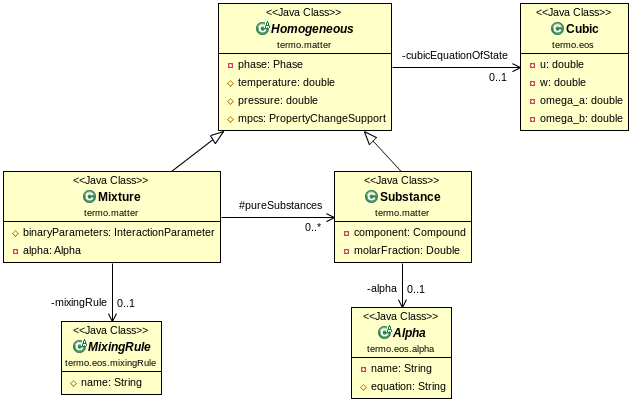
\includegraphics[scale=0.7]{homogeneousCalculations.png}
    \caption{Estructura de la librería para el cálculo de propiedades.}
    \label{fig:homogeneousCalculations}
\end{figure}

Nótese de la figura \ref{fig:homogeneousCalculations} los siguiente:
\begin{itemize}
	\item Que la clase `Homogeneous' contiene una ecuación del tipo `Cubic'.
 	\item Que las clases `Substance' y `Mixture' heredan las propiedades de la clase `Homogenous', como la ecuación cúbica, y puede hacer uso de ella.

\end{itemize}

	Cualquiera de las dos implementaciones de la clase `Homogeneous' tiene los métodos necesarios para calcular los parámetros de la ecuación cúbica según el código \ref{lst:homogeneousParameters}.

\begin{lstlisting}[caption=Cualquier objeto tipo `Homogeneous' puede calcular los parámetros de la ecuación de estado cúbica a y b, label={lst:homogeneousParameters}]
	Homogeneous homogeneous = ...// Objeto tipo `Homogeneous'.
	double a = homogeneous.calculate_a_cubicParameter();
	double b = homogeneous.calculate_b_cubicParameter();
\end{lstlisting}


\subsection{Compuesto puro}\label{subsec:substance}

Como se muestra en la figura \ref{fig:homogeneousCalculations} la clase `Substance' continene una expresión de $\alpha$, y una ecuación de estado, necesarias para realizar el cáculo de los parámetros, segun las ecuaciones \ref{eq:a} y \ref{eq:b}. 

La expresión de $\alpha$ puede ser una función de la temperatura, las expresiones implementadas en el presente trabajo se muestran en la tabla \ref{tab:alphas}.

\begin{table}[!h]
	\centering
	\caption{Expresiónes de $\alpha$ disponibles en la librería}\label{tab:alphas}
	\begin{tabular}{|c|c|c| }
		\hline
		Expresión & Parámetros & Ecuación de estado\\
		\hline
		Soave    &  ---& PR\\
		Peng and Robinson & ---& PR \\
		Mathias & $A$ & SRK\\
		Stryjek and Vera & $k_1$ & PRSV\\
		Adachi and Lu & $A,B$&SRK,PR\\
		Soave & $A,B$&SRK,PR\\
		Melhem, et al. & $A,B$&SRK,PR\\
		Androulakis et al. & $A,B,C$& SRK,PR\\
		Mathias and Copeman & $A,B,C$& SRK,PR\\
		Yu and Lu & $A,B,C$&SRK,PR\\
		Stryjek and Vera & $A,B,C$&PR\\
		Twu & $L,M,N$&TST\\
		Twu & ---&TST,PR\\
		GCEOS & ---& (Cualquier u y w)\\
		\hline
	\end{tabular}
\end{table}
\subsubsection{Creación de un objeto tipo `Substance'}\label{subsub:substanceCreation}

Es necesario utilizar el método constructor de la clase `Substance' para crear un objeto de este tipo, se debe proporcionar como parámetros la ecuación de estado deseada, la exprsión de $\alpha$, una instancia de la clase `Compound' como se muestra en la sección \ref{sec:compounds} y la fase de la substancia.

En la sección \ref{subsec:cubicCreation} se mostró como crear una ecuación de estado cúbica previamente definida, a través de la clase `EquatiosOfState'. Los valore de $\Omega_a$ y $\Omega_b$ se muestran en la tabla \ref{tab:cubics}. De forma muy similar al de las ecuaciońes de estado,la selección de la expresión de $\alpha$ se realiza a través de la clase `Alphas'.

El código \ref{lst:substanceCreation} muestra como crear una objeto del tipo substancia.

\begin{lstlisting}[caption={Creación de un objeto tipo `Substance' para el compuesto Ciclohexano, con la ecuación de estado Soave Redlich Kwong y la expresión de $\alpha$ de mathias },label={lst:substanceCreation}]

Compound compound = new Compound("Cyclohexane");
compound.setCriticalPressure(4073000);
compound.setCriticalTemperature(553.5);
compound.setAcentricFactor(0.211);


Cubic srk = EquationsOfState.redlichKwongSoave();
Alpha mathias = Alphas.getMathiasExpression();


Substance substance = new Substance(srk,mathias, compound,Phase.LIQUID);
\end{lstlisting}

	Finalmente se utiliza el objeto creado para realizar el cálculo de los parámetros de la ecuación de estado cúbica, en el código \ref{lst:substanceParams}.

\begin{lstlisting}[caption={Cálculo de los parámetros para la ecuación de estado cúbica con la clase `Substance'.},label={lst:substanceParams}]
double a = substance.calculate_a_cubicParameter();
double b = substance.calculate_b_cubicParameter();
\end{lstlisting}
 

Nótese que el código \ref{lst:homogeneousParameters} y el código \ref{lst:substanceParams} es idéntico y aunque parece redundate, solo se muestra para señalar el polimorfismo de la librería , es decir que el objeto substance es del tipo `Homogeneous' además del tipo `Substance', y tiene accesso a los métodos en las dos clases.


\subsubsection{Mezcla}\label{subsec:mixture}

El cálculo de los parámetros para una mezcla depende de la regla de mezclado, y en el caso de las reglas de mezclado basadas en la energía libre de exceso, también del modelo de actividad.

Las reglas de mezclado incluidas en este trabajo se muestran en la tabla \ref{tab:mixingrules}, y los modelos de actividad se listan en la tabla \ref{tab:activitymodels}.

\begin{table}[!h]
	\caption{Reglas de mezclado implementadas}\label{tab:mixingrules}
	\begin{tabularx}{\textwidth}{|X|X|X|}
		\hline
		Regla & Parámetros & \\
		\hline
		Van Der Waals & $k_{ij}$ & $k_{ij} = k_{ji}$ \\
		Mathias-Klotz-Prausnitz& $k_{ij}$ & $k_{ij} \neq k_{ji}$ \\
		Huron Vidal & Según el model de actividad & \\
		Wong Sandler & $k_{ij}$ + los parámetros del modelo de actividad & $k_{ij} = k_{ji}$ \\
		\hline
	\end{tabularx}
\end{table}

\begin{table}[!h]
	\caption{Modelos de actividad }\label{tab:activitymodels}
	\begin{tabularx}{\textwidth}{|X|X|X|}
		\hline
		Modelo de actividad & Parámetros & \\
		\hline
		Wilson & $a_{ij}$, $b_{ij}$  & \\
		NRTL & $a_{ij}$, $b_{ij}$, $\alpha_{ij}$ & $\alpha_{ij} = \alpha_{ji}$ \\
		\hline
	\end{tabularx}
\end{table}
\subsubsection{Creación de un objeto tipo `Mixture'}\label{subsub:mixtureCreation}

Un objeto tipo `Mixture' contiene dentro de sí un conjuto de objetos tipo `Substance', esto hace que su creación sea mas compleja. Se ha escrito la clase `MixtureBuilder' para facilitar la creación de los objetos de la clase `Mixture'.

La clase `MixtureBuilder' facilita la creación de los objetos `Substance' que forman el conjunto de compuestos de la mezcla, y permite asignar una expresión de $\alpha$ diferente para cada compuesto.

El código \ref{lst:mixturecreation} muestra la creación de una mezcla, donde la expresión de $\alpha$ es la misma para cada compuesto puro. 

\begin{lstlisting}[caption={Creación de una mezcla con la clase `MixtureBuilder' asignando la misma expresión de $\alpha$ para cada compuesto puro.}, label={lst:mixturecreation} ]

Compound cyclohexane = new Compound("Cyclohexane");
cyclohexane.setCriticalPressure(4073000);
cyclohexane.setCriticalTemperature(553.5);
cyclohexane.setAcentricFactor(0.211);

Compound pentane = new Compound("N-pentane");
pentane.setCriticalPressure(3370000);
pentane.setCriticalTemperature(469.7);
pentane.setAcentricFactor(0.251);

Cubic equationOfState = EquationsOfState.pengRobinson();
Alpha alpha = Alphas.getMathiasAndCopemanExpression();

Mixture mixture = new MixtureBuilder()
			.addCompounds(cyclohexane,pentane)
			.setAlpha(alpha)
			.setEquationOfState(equationOfState)
			.setPhase(Phase.VAPOR)
			.build();

\end{lstlisting}

Es posible crear la mezcla con una expresión de $\alpha$ diferente para cada compuesto puro según el código \ref{lst:mixtureParametersDifAlphas}. 


\begin{lstlisting}[caption={Código para el cálculo de los parámetros de la ecuación de estado en una mezcla, con diferentes expresiones de $\alpha$},label={lst:mixtureParametersDifAlphas}]
Mixture mixture = new MixtureBuilder()
			.addCompound(cyclohexane,Alphas.getPengAndRobinsonExpression())
			.addCompound(pentane,Alphas.getStryjekAndVeraExpression())
			.setEquationOfState(eos)
			.setPhase(phase)
			.setMixingRule(mixingRule)
			.setInteractionParameter(k)
			.build();
\end{lstlisting}

Finalmente se pueden calcular los parámetros de la ecuación cúbica con el código \ref{lst:mixtureParameters}.

\begin{lstlisting}[caption={Cálculo de parámetros de la mezcla},label={lst:mixtureParameters}]
double a = mixture.calculate_a_cubicParameter();
double b = mixture.calculate_b_cubicParameter();
\end{lstlisting}
%hecho
		\section{Ecuación de capacidad calorífica}\label{sec:cp}

	Los cálculos de entalpía y entropía necesitan de una ecuación de capacidad calorífica.

	La librería \Materia  define una interface para obligar que todas las implementaciones de la ecuación tengan los métodos para calcular la entalpía y entropía del gas ideal según la ecuaciones \ref{eq:idealgasenthalpy}, \ref{eq:idealgasentropy}.

	Incluidas para el presente trabajo la librería \Materia implementa las ecuaciones 107 del DIPPR y una ecuación Polinomial obtenida de la base de datos Chemsep ver ecuaciones \ref{eq:dippr107} y \ref{eq:chempse16}.
	
	Predeterminadamente se usa la ecuación 107 de DIPPR.
		\section{Materia homogénea}\label{sec:homogeneous}

	La clase `Homogeneous' representa a las substancias o mezclas que se encuentran en una sola fase, las propiedades que se pueden calcular de una fase son: 
\begin{itemize}
	\item fugacidad
	\item presión
	\item factor compresibilidad 
	\item volume molar
	\item entalpía 
	\item entropía 
	\item energía libre de gibbs.
\end%hecho			
		\section{Equilibrio Líquido-Vapor}\label{sec:heterogeneous}

	La clase `Heterogeneous' se encarga de los cálculos de equilibrio entre las fases líquido y vapor. La clase contiene dos instancias de la clase `Homogeneous' que representan a la clase líquida y a la clase vapor. La clase implementa los algoritmos numéricos para igualar los cálculos de la fugacidad entre las fases.

	Los cálculos de equilibrio que se implementan en este trabajo son:

	\begin{itemize}

		\item Substancias
			\begin{itemize}
				\item Temperatura de saturación.
				\item Presión de saturación.
			\end{itemize}

		\item Mezclas
	\begin{itemize}
		\item Presión de burbuja, sección \ref{subsec:bubblepressure}.
		\item Presión de rocío, sección \ref{subsec:dewpressure}.
		\item Temperatura de burbuja, sección \ref{subsec:bubbletemperature}.
		\item Temperatura de rocío, sección \ref{subsec:dewtemperature}.
		\item Flash temperatura-presión \ref{subsec:flash}.
	\end{itemize}

	\end{itemize}

	Los algoritmos son muy similares, las principales diferencias consisten en la función objetivo.

	La clase `HeterogeneousSubstance' realiza los cálculos de equilibrio para las substancias y la clase `HeterogeneousSubstance' realiza los cálculos de equilibrio para las mezclas, en la figura \ref{fig:heterogeneous} ser muestra la estructura.

\begin{figure}[!h]
  \centering
    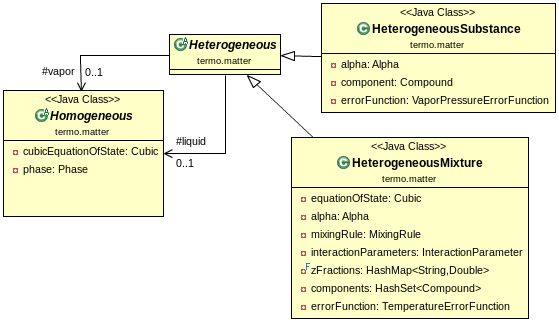
\includegraphics[scale=0.7]{heterogeneous.png}
    \caption{Estructura de la librería para el cálculo de equilibrio Líquido-Vapor.}
    \label{fig:heterogeneous}
\end{figure}

	Los cálculos de la presente sección se realizan de forma muy similar, primero indicando la variable conocida con el método `set', después invocando el método que realiza el algoritmo para conocer la incognita, el método puede recibir o no un estimado inicial y finalmente obtener el resultado de la variable con el método `get'.

	Cada sección muestra el uso de la librería con fragmentos de código que realizan el cálculo con y sin el estimado inicial. También se indica que método se usa para estimar la varible incognita en caso de no proporcionar un estimado inicial.

		
%hecho			
		\section{Estimación de parámetros}\label{sec:optimization}

	Para el cálculo del parámetro $a$ de la ecuación de estado cúbica es necesaria una expresión de $\alpha$ como se muestra en la ecuación \ref{eq:a}. Todas las expresiones de $\alpha$ escritas para este trabajo se listan en la tabla \ref{tab:alphas}. Estas expresiones pueden tener parámetros que deben ser estimados en base a datos experimentales de compuestos puros. La estimación de los parámetros de $\alpha$ se realiza en la clase `HeterogeneousSubstance'.

	Para realizar el cálculo de los parámetros de le ecuación cúbica para una mezcla, es necesario utilizar una regla de mezclado como se mostró en la sección \ref{subsec:mixture}. Las reglas de mezclado escritas para este trabajo se listan en la tabla \ref{tab:mixingrules}. Las reglas de mezclado usan parámetros que deben ser estimados en base a datos experimentales de mezclas binarias. La estimación de los parámetros binarios se realiza en la clase `HeterogeneousMixture'.

	\begin{itemize}
		\item{Sección} \ref{subsec:alphaoptim} Estimación de parámetros de la expresión de $\alpha$.
		\item{Sección} \ref{subsec:binaryoptim} Estimación de parámetros de interacción binaria para las reglas de mezclado.
	\end{itemize}

	





%hecho


	\chapter{Página de Internet}\label{chap:webPage}

	Una gran ventaja del lenguaje java es su capacidad para crear páginas de internet. En el presente trabajo se creó una página de internet cuyo objetivo es exponer las funciones principales de la librería materia.

	La página se encuentra en la dirección web: \url{chimicae-materia.rhcloud.com}, se recomienda utilizar un navegador moderno como google chrome o mozilla firefox.

	El presente capítulo trata sobre como utilizar la página para:

	\begin{itemize}
		\item{Crear}
			\begin{itemize}
				\item{Substancias} Sección \ref{sec:webSubstanceCreator}
				\item{Mezclas} Sección \ref{sec:webMixtureCreator}
			\end{itemize}
		\item{Gráficas}
			\begin{itemize}
				\item \nameref{subsec:pvt} \ref{subsec:pvt}
				\item \nameref{subsec:zpt} \ref{subsec:zpt}
				\item \nameref{subsec:fpt} \ref{subsec:fpt}
				\item {A partir del envolvente de fases}
				\begin{itemize}
					\item {Envolvente de fases} \ref{subsec:envelope}
					\item \nameref{subsec:tep} \ref{subsec:tep}
					\item \nameref{subsec:tsp} \ref{subsec:tsp}
					\item \nameref{subsec:tgp} \ref{subsec:tgp}
				\end{itemize}
				% \item \nameref{subsec:tpv}
			\end{itemize}
		\item{Estimación de parámetros}
			\begin{itemize}
				\item Expresión de $\alpha$
				\item Regla de Mezclado
			\end{itemize}
	\end{itemize}

	La página de internet contiene las instrucciones con mas detalle en la página de inicio.

\section{Selección de compuestos puros}\label{sec:webCompounds}

	La página de internet dispone de la base de datos ChemSep v6.96 derechos de autor  Harry Kooijman y Ross Taylor (2013) bajo la licencia `Artistic License': \url{ http://www.perlfoundation.org/artistic_license_2_0}, que contiene 432 compuestos, el archivo orginal puede ser consultado en la url \url{https://raw.githubusercontent.com/HugoRedon/chimicae/master/src/main/resources/data/chemsep1.xml}.

	Primero se deben cargar los compuestos puros en la sección `Creación' - `Compuesto Puro'. Para buscar compuestos se debe escribir el nombre en inglés del compuesto deseado en el recuadro de texto al lado de la etiqueta `Buscar'. Al dar click en el boton buscar la página buscará coincidencias entre el nombre escrito y los nombres de la base de datos. Los compuestos que muestren coincidencia con el texto escrito se mostrarán en una lista debajo del recuadro.

	Para agregar un compuesto de la lista basta con dar click en el boton `Agregar' junto al nombre del compuesto. En la tabla a la derecha de la página se muestran los compuestos agregados. Ver la figura \ref{fig:pureCompounds}.

	\begin{figure}[H]
		\centering
		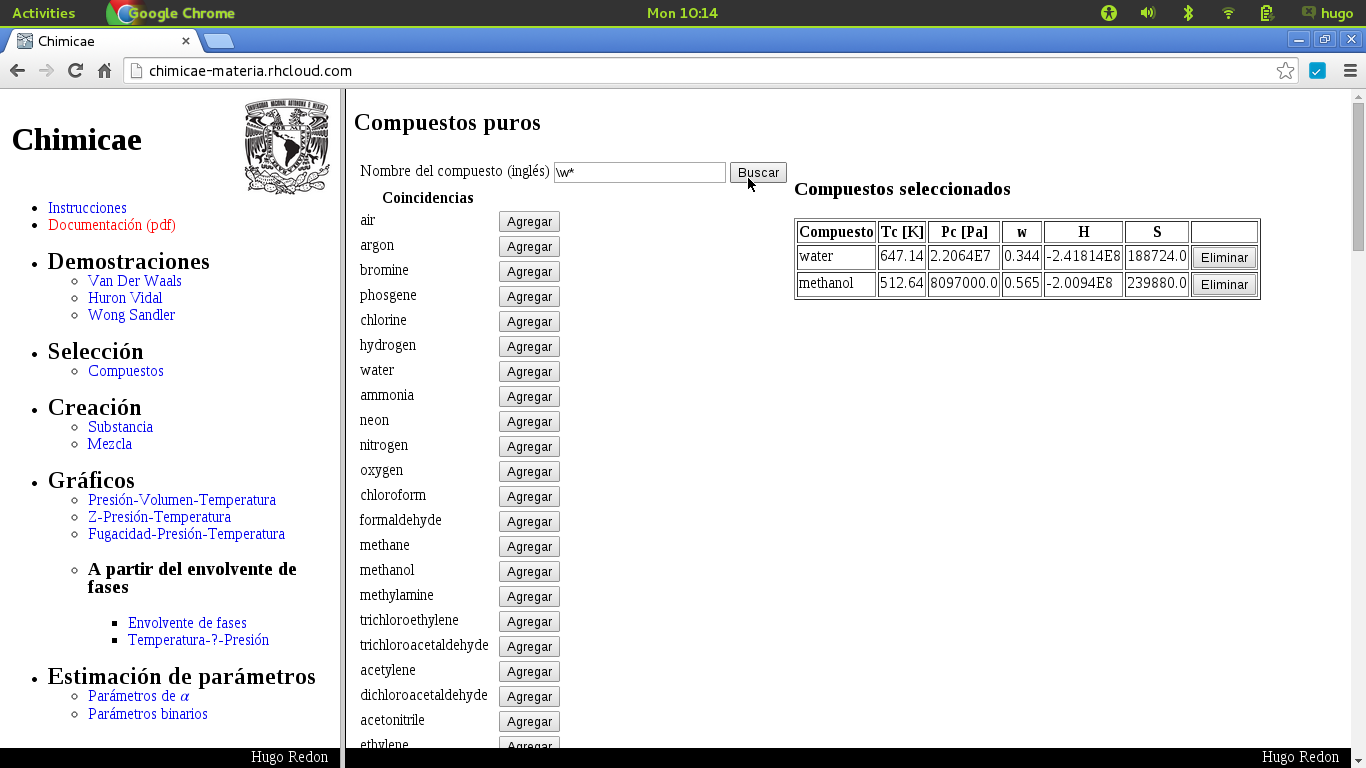
\includegraphics[scale=0.34]{pureCompounds.png}
		\caption{Formulario para seleccionar y cargar compuestos puros en la página de internet}
		\label{fig:pureCompounds}
	\end{figure}

\section{Creación de substancias}\label{sec:webSubstanceCreator}
	
	En la sección `Creación' - `Substancia' se permite crear materia de un solo compuesto, para después utilizarse en las secciones de graficación y estimación de parámetros de la expresión de $\alpha$.

	Esta sección permite elegir la ecuación cúbica, la expresión de $\alpha$, el compuesto y la fase homogéna con la cual se creará la substancia. Al final de la sección el botón `Aceptar' creará la Substancia y mostrará un resumen de la substancia creada.

	La figura \ref{fig:substanceCreator} muestra la interfaz de usuario para la creación de substancias. La figura \ref{fig:substanceProperties} muestra las propiedades de la substancia creada.

	\begin{figure}[H]
		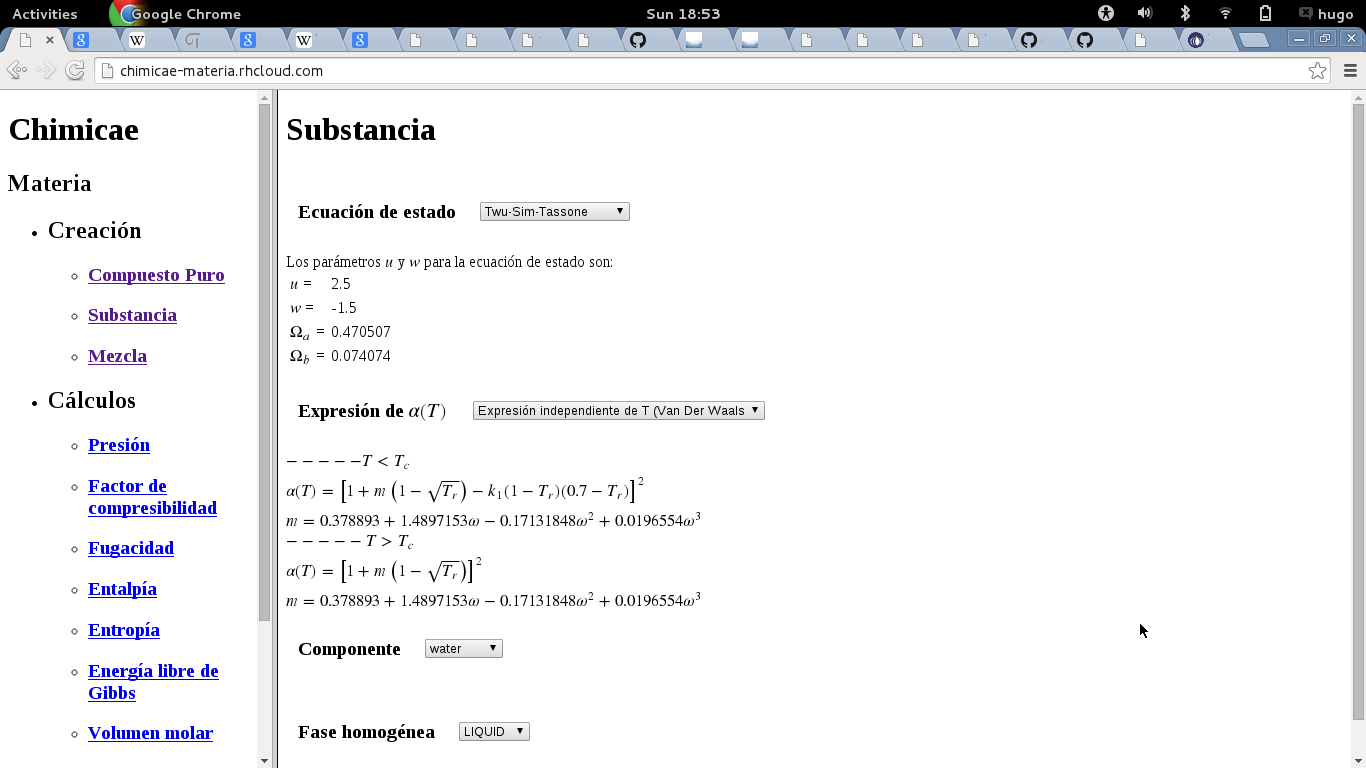
\includegraphics[scale=0.3]{substanceCreator.png}
		\caption{Formulario para crear substancias en la página de internet}
		\label{fig:substanceCreator}
	\end{figure}

	\begin{figure}[H]
		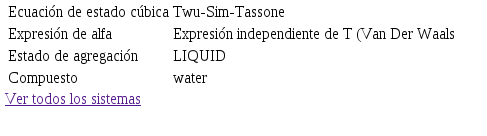
\includegraphics[scale=0.3]{substanceProperties.png}
		\caption{Página que muestra las propiedades de la substancia recien creada}
		\label{fig:substanceProperties}
	\end{figure}

\section{Formación de Mezclas}\label{sec:webMixtureCreator}

	En la sección `Creación' - `Mezcla' se permite crear mezclas con varios compuestos.Para la sección de estimación de parámetros binarios \ref{sec:webBinaryOptim} solo estarán disponibles aquellas mezclas que contengan dos compuestos.

	El formulario permite elegir la ecuación cúbica, la fase ,la regla de mezclado, permite elegir cada compuesto, definir su expresión de $\alpha$ y su fración molar. Ver figura \ref{fig:webMixCreator}.

	\begin{figure}[H]
		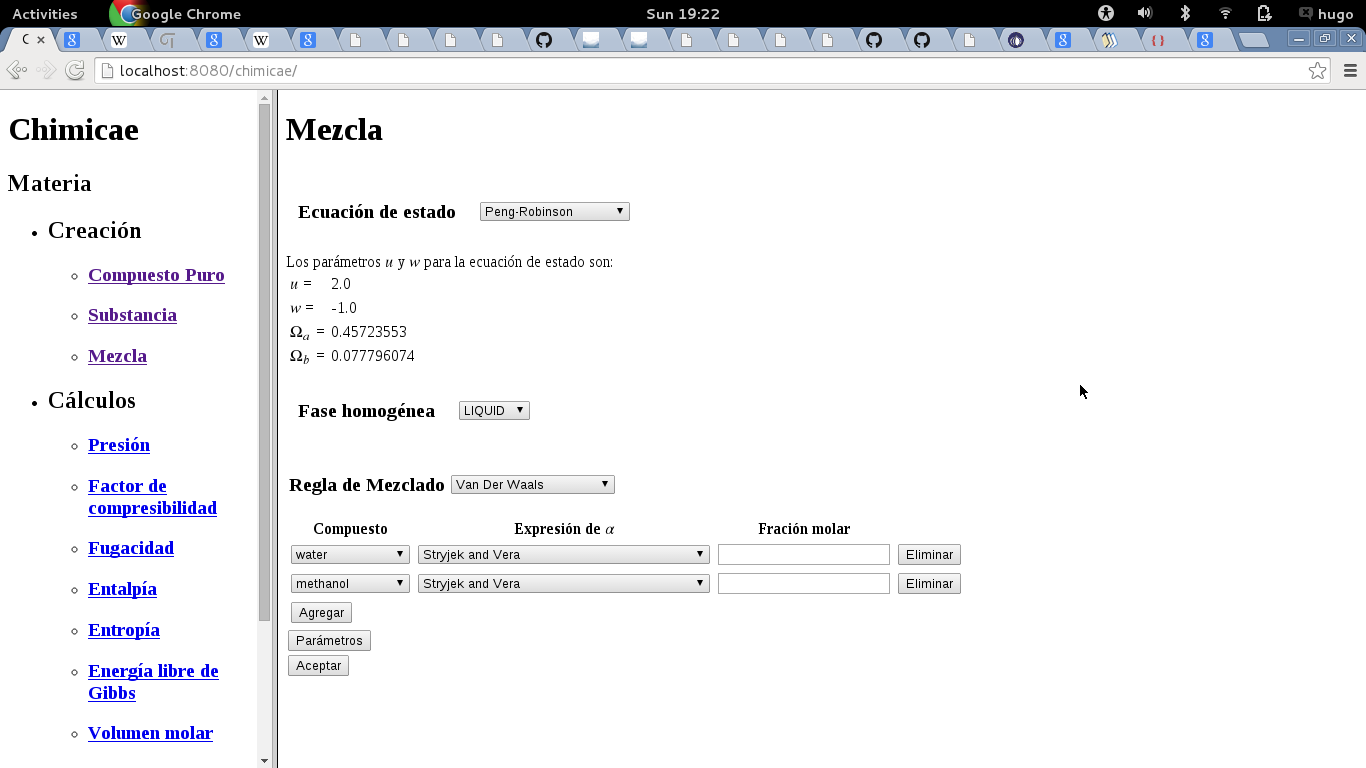
\includegraphics[scale=0.3]{mixtureCreator.png}
		\caption{Formulario para la creación de mezclas}
		\label{fig:webMixCreator}
	\end{figure}

	El botón con la etiqueta `Parámetros' permite definir los parámetros binarios para la regla de mezclado seleccionada. Finalmente el botón `Aceptar' construye la mezcla y la pone a disposición para las siguientes secciones.

\section{Gráficos}

	Las secciónes de gráficos dividen el recuadro derecho de forma horizontal, en la parte superior se localizan los controles de las gráficas, y en la parte inferior la gŕafica tridimensional.

	En esta sección estan disponibles las substancias y mezclas creadas anteriormente, basta con dar click en la caja tipo `combobox' y seleccionar el sistema, esto es igual para todas las gráficas de la sección.

	En algunas gráficas se muestran los resultados de la fase líquida y vapor sin importar la fase seleccionada en el momento de la creación del sistema.

	\subsection{Gráficos Presión-Volumen-Temperatura}\label{subsec:pvt}
		En este tipo de gráfica no se involucra la fase del sistema seleccionada previamente. 

		La sección de controles permite elegir el rango del volumen molar y el rango de temperatura.
		
		La figura \ref{fig:press} muestra el diagrama tridimensional presión-volumen-temperatura creado en la página de internet.
		\begin{figure}[H]
			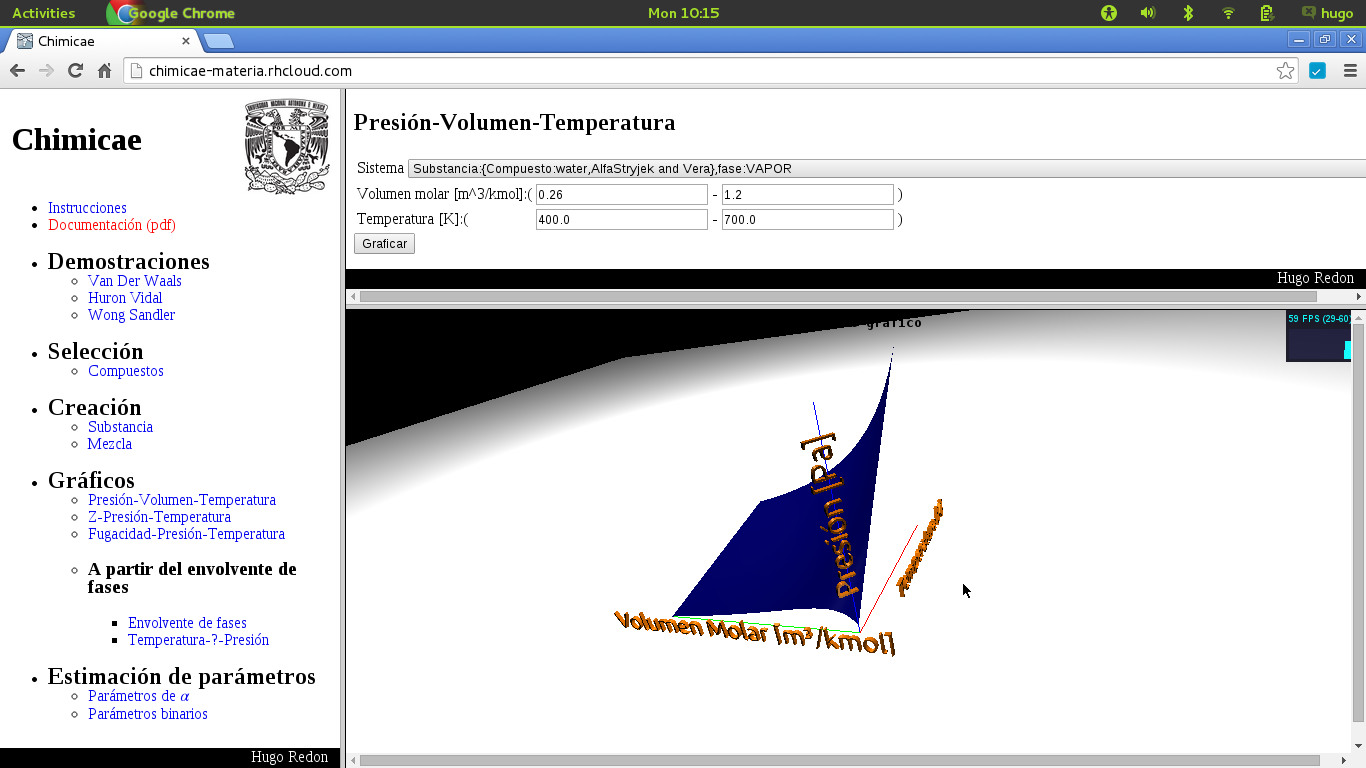
\includegraphics[scale=0.3]{waterPressurePlot.png}
			\caption{Gráfica de presión-volumen-temperatura para el agua con la ecuación de estado de Peng-Robinson y la expresion de $\alpha$ de Stryjek and Vera que esta cargada por default. El rango de volumen: $0.26-1.2 [\frac{m^3}{kmol}]$ y temperatura:$400-700[K]$ }
			\label{fig:press}
		\end{figure}
	\subsection{Gráficos Z-Presión-Temperatura}\label{subsec:zpt}
		Usualmente las gráficas del factor de compresibilidad se crean en dos dimensiones mostrando diferentes temperaturas en el mismo plano y no es posible ver efecto que se tiene a altas temperaturas y presiones.

		Esta gráfica depende de la fase seleccionada para el sistema.

		Semejante a la sección anterior se debe determinar un rango de presión y temperatura. La figura \ref{fig:zplot} muestra el efecto en tercera dimensión.
		\begin{figure}[H]
			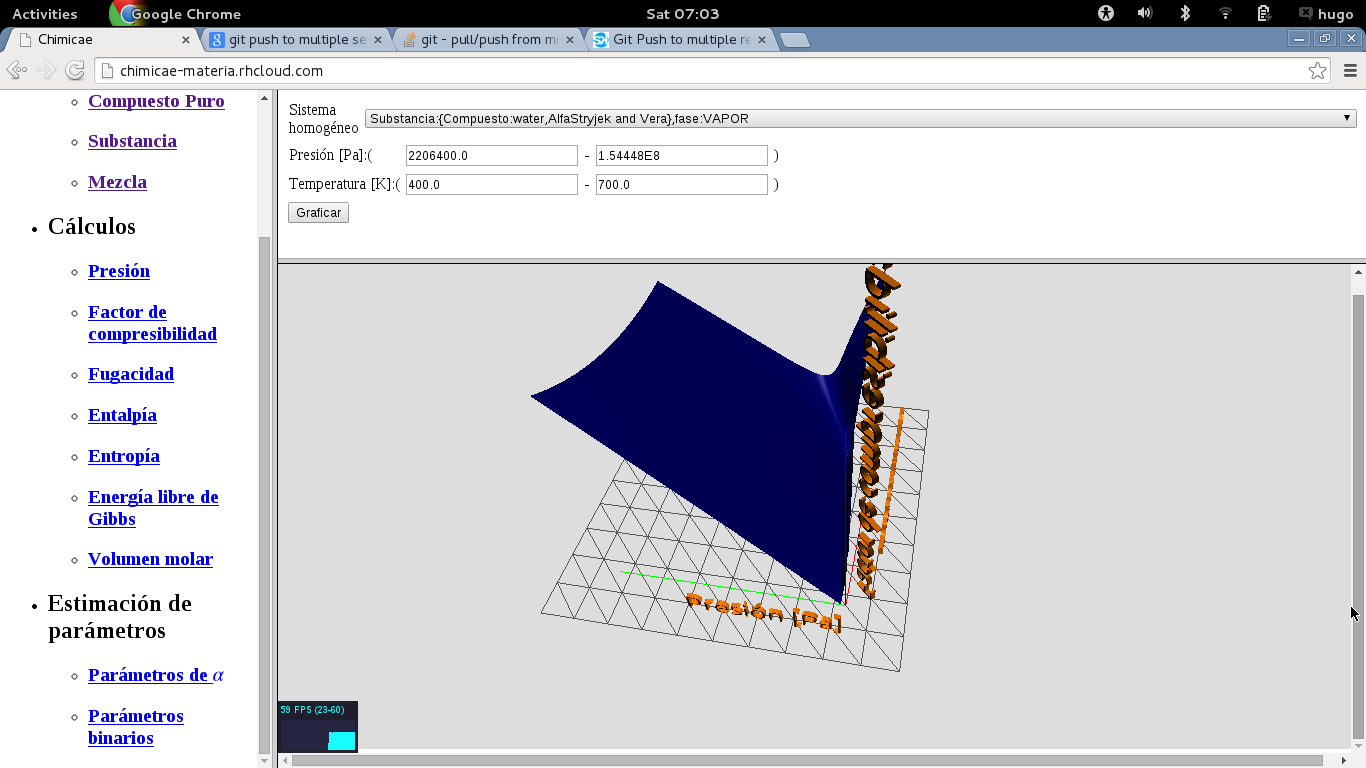
\includegraphics[scale=0.3]{waterZPlot.png}
			\caption{Gŕafica de z(Factor de compresibilidad)-Presión-Temperatura para el agua con la ecuación de estado de Peng-Robinson y la expresiónde $\alpha$ Stryjek and Vera.}
			\label{fig:zplot}
		\end{figure}
	\subsection{Gráficos Fugacidad-Presión-Temperatura}\label{subsec:fpt}

		En esta gráfica se dibujan las curvas de fugacidad para las dos fases, para el líquido (rojo) y el vapor (azul).

		El objetivo de la gráfica es observar el equilibrio líquido-vapor en la línea de intersección de los planos. Ver la figura \ref{fig:fugplot}.

		La línea de equilibrio (Intersección de los planos) puede aparecer o no, dependiendo del dominio elegido.

		\begin{figure}[H]
			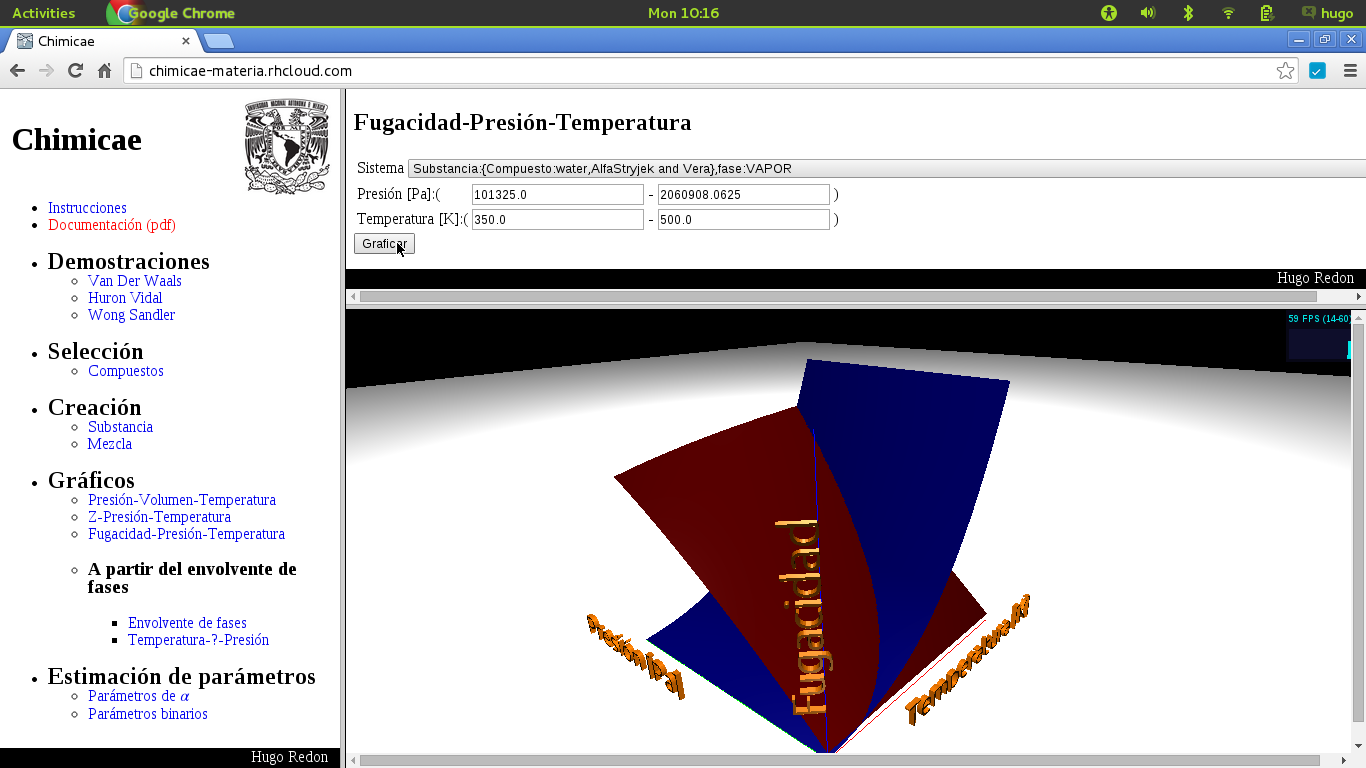
\includegraphics[scale=0.3]{waterFugacityPlot.png}
			\caption{Gŕafica de Fugacidad-Presión-Temperatura para el agua con la ecuación de estado de Peng-Robinson y la expresión de $\alpha$ stryjek y Vera}
			\label{fig:fugplot}
		\end{figure}

	\subsection{Gráficos a partir del envolvente de fases}\label{subsec:envelope}
		Para crear los siguientes diagramas es necesario calcular la envolvente de fases y a partir de éste se calculan las demás propiedades.

	\subsubsection{Envolvente de fases}
		Para crear la envolvente basta con elegir el sistema deseado y dar click en el botón. En el diagrama se muestra la envolvente de la mezcla y se agregan las curvas de Presión de vapor-Temperatura de los compuestos puros, ver la figura \ref{fig:envelope}
		\begin{figure}[H]
			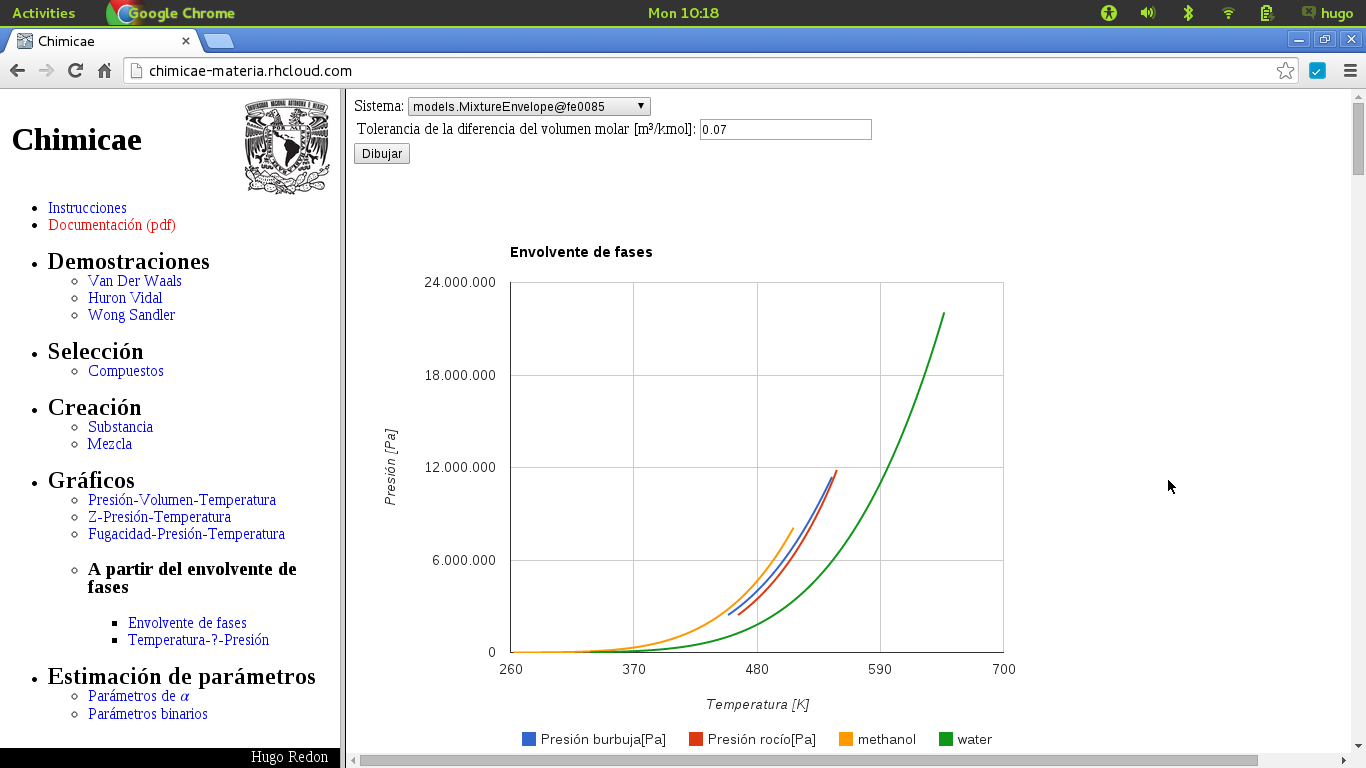
\includegraphics[scale=0.3]{envelope.png}
			\caption{Gráfica del envolvente de fases Presión-Temperatura para el sistema  agua metanol con la ecuación de estado de Peng-Robinson y la expresión de $\alpha$ stryjek y Vera}
			\label{fig:envelope}
		\end{figure}

	\subsubsection{Gráficos Temperatura-Entalpía-Presión}\label{subsec:tep}
		Una vez calculado la envolvente de fases las propiedades se calculan para la fase vapor y la fase líquida.

		En esta gráfica no se debe determinar el rango, ya que éste se calculó en el envolvente de fases.

		Podemos ver la forma de la gráfica en la figura \ref{fig:hplot}.

		\begin{figure}[H]
			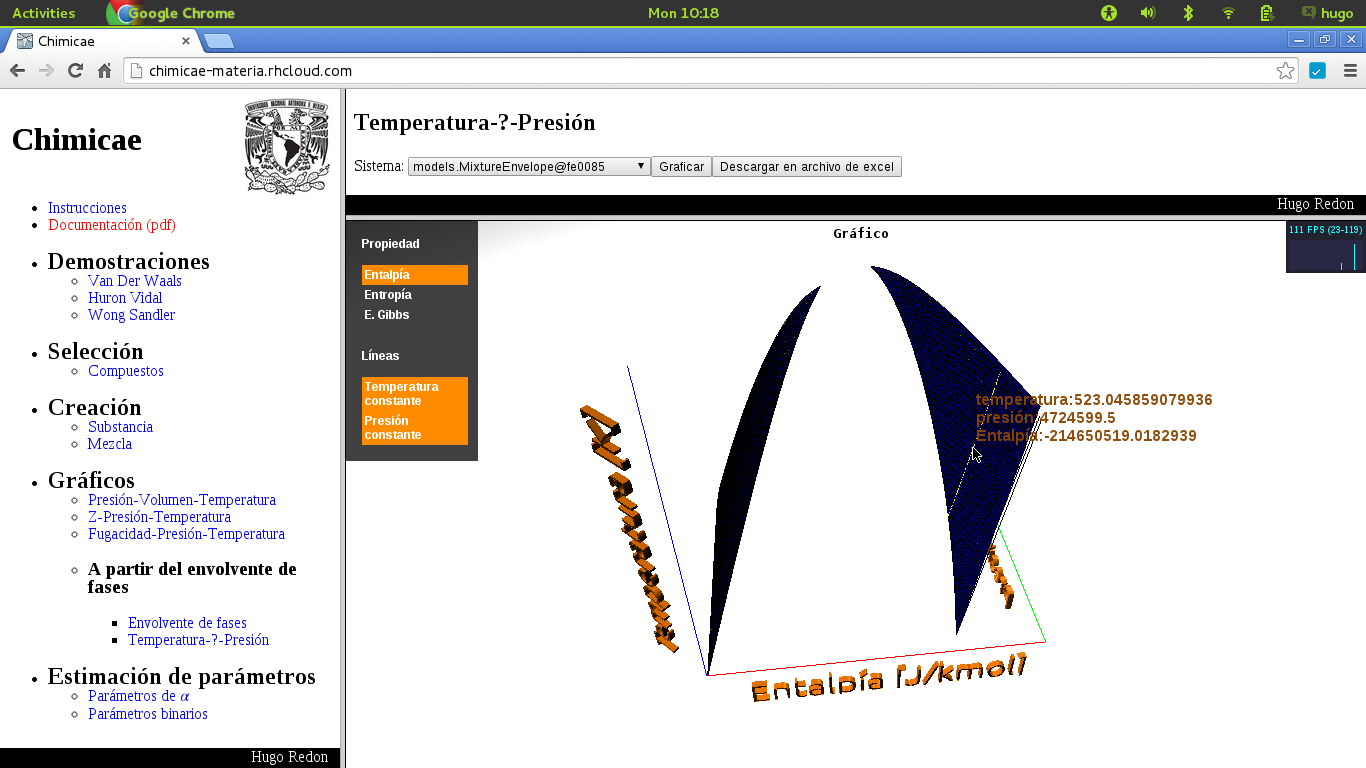
\includegraphics[scale=0.3]{waterEnthalpyPlot.png}
			\caption{Gráfica de Temperatura-Entalpía-Presión para el agua con la ecuación de estado de Peng-Robinson y la expresión de $\alpha$ stryjek y Vera}
			\label{fig:hplot}
		\end{figure}
	\subsubsection{Gráficos Temperatura-Entropía-Presión}\label{subsec:tsp}	
		\begin{figure}[H]
			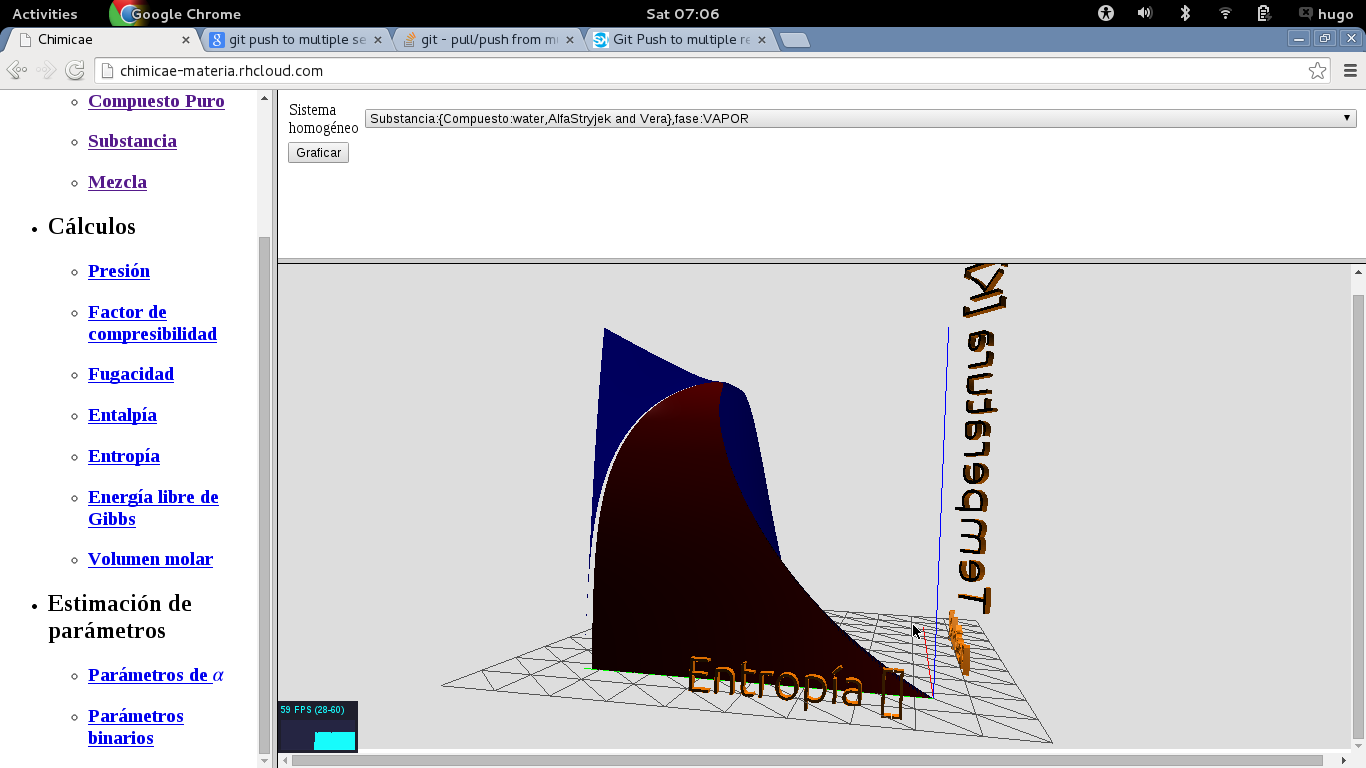
\includegraphics[scale=0.3]{waterEntropyPlot.png}
			\caption{Gráfica de Temperatura-Entropía-Presión para el agua con la ecuación de estado de Peng-Robinson y la expresión de $\alpha$ Stryjek y Vera}
			\label{fig:splot}
		\end{figure}
	\subsubsection{Gráficos Temperatura-Gibbs-Presión}\label{subsec:tgp}
		\begin{figure}[H]
			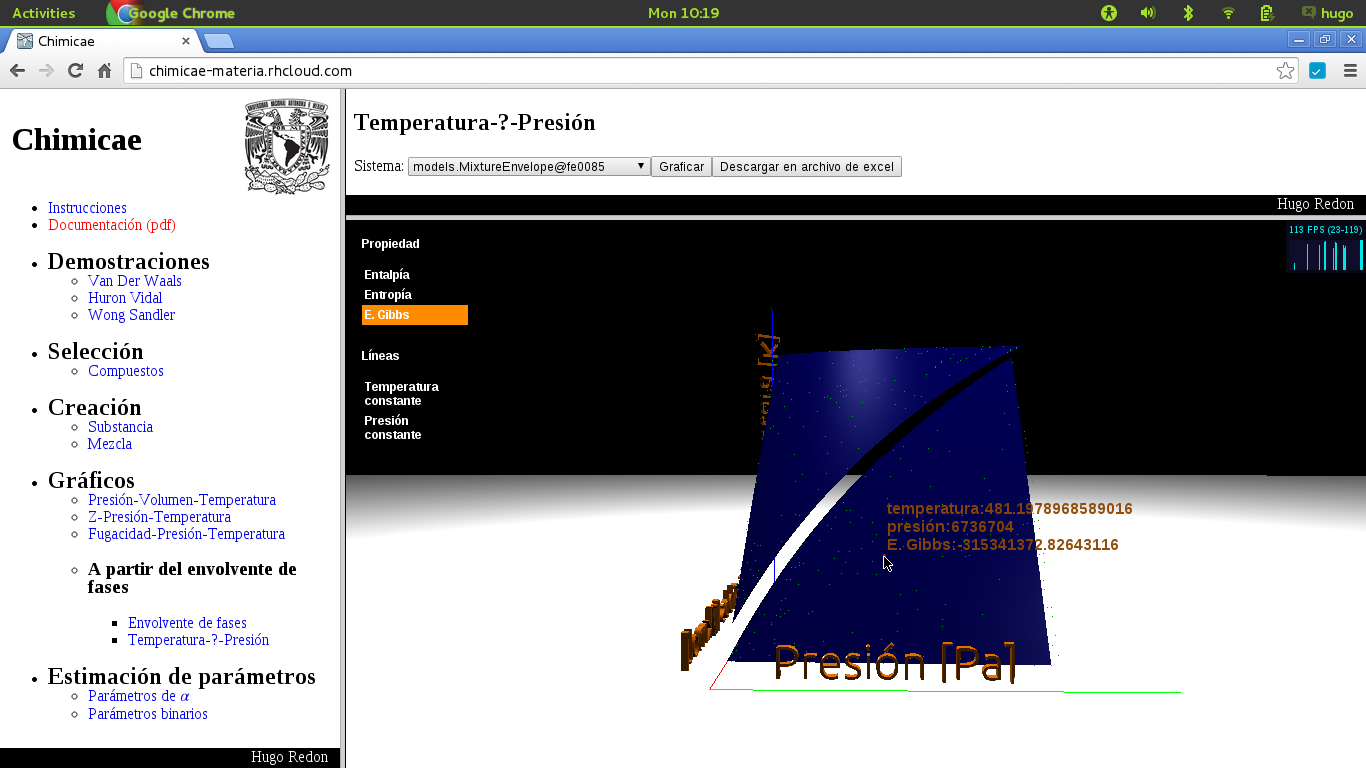
\includegraphics[scale=0.3]{waterEGPlot.png}
			\caption{Gráfica de Temperatura-(Energía libre de Gibbs)-Presión para el agua con la ecuación de estado de Peng-Robinson y la expresión de $\alpha$ de Stryjek y Vera}
			\label{gplot}
		\end{figure}
	% \subsection{Temperatura-Presión-Volumen}\label{subsec:tpv}
	% 	\begin{figure}[H]
	% 		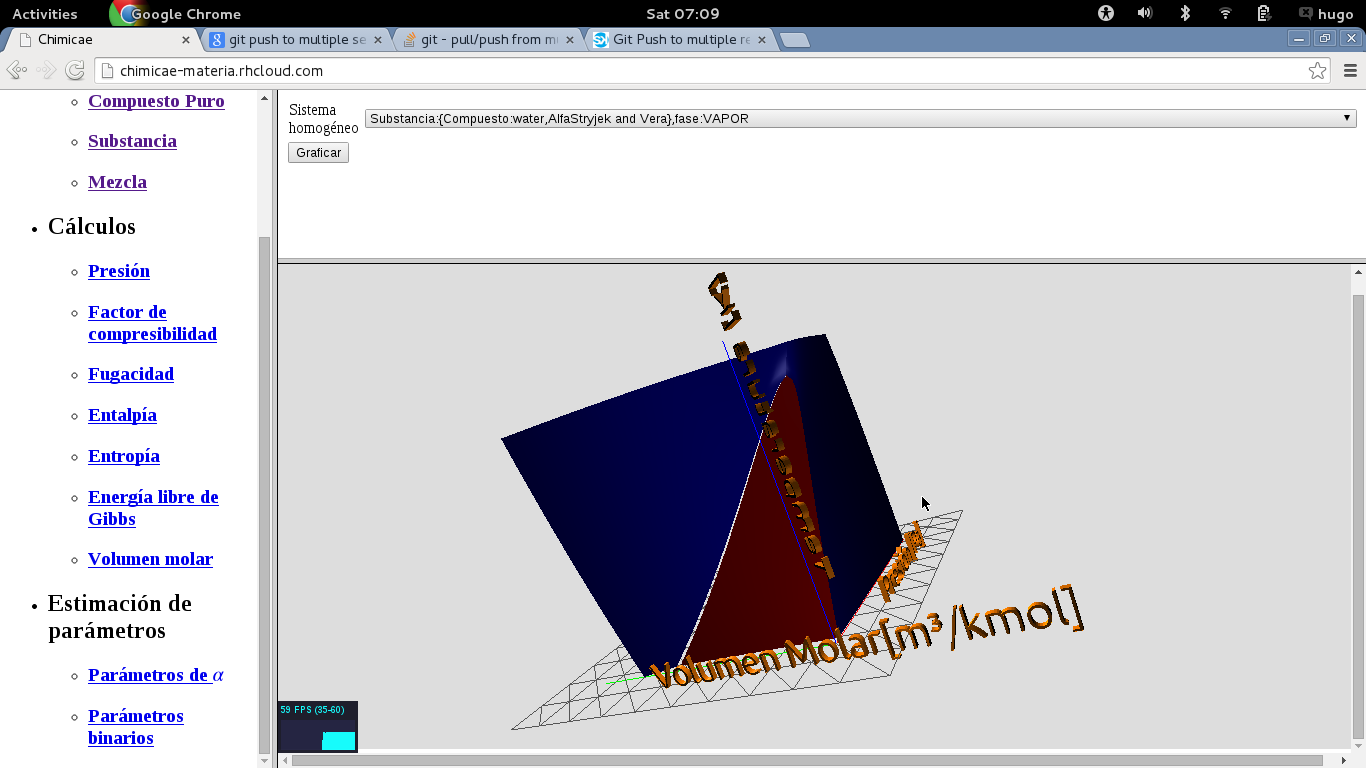
\includegraphics[scale=0.3]{waterVolumePlot.png}
	% 		\caption{Gráfica de Temperatura-Presión-Volumen molar para el agua con la ecuación de estado de Peng-Robinson y la expresión de $\alpha$ de Stryjek y Vera}
	% 		\label{vplot}
	% 	\end{figure}
	
	
\section{Estimación de parámetros de $\alpha$}\label{sec:webAlphaOptim}
	En la sección de `Estimación de parámetros' - `Parámetros de $\alpha$' pódemos seleccionar una de las substancias creadas y estimar sus parámetros con una serie de datos generados a través de la ecuación \ref{eq:101vaporpressure} que nos proporciona la base de datos Chemsep.

	En la sección se muestra una gráfica que compara el modelo con los datos generados, una gráfica que muestra el error relativo, y finalmente una gráfica que muestra la historia de convergencia de la estimación de los parámetros.

	Una imagen del formulario se presenta en la figura \ref{fig:alphaOptim}

\begin{figure}[H]
	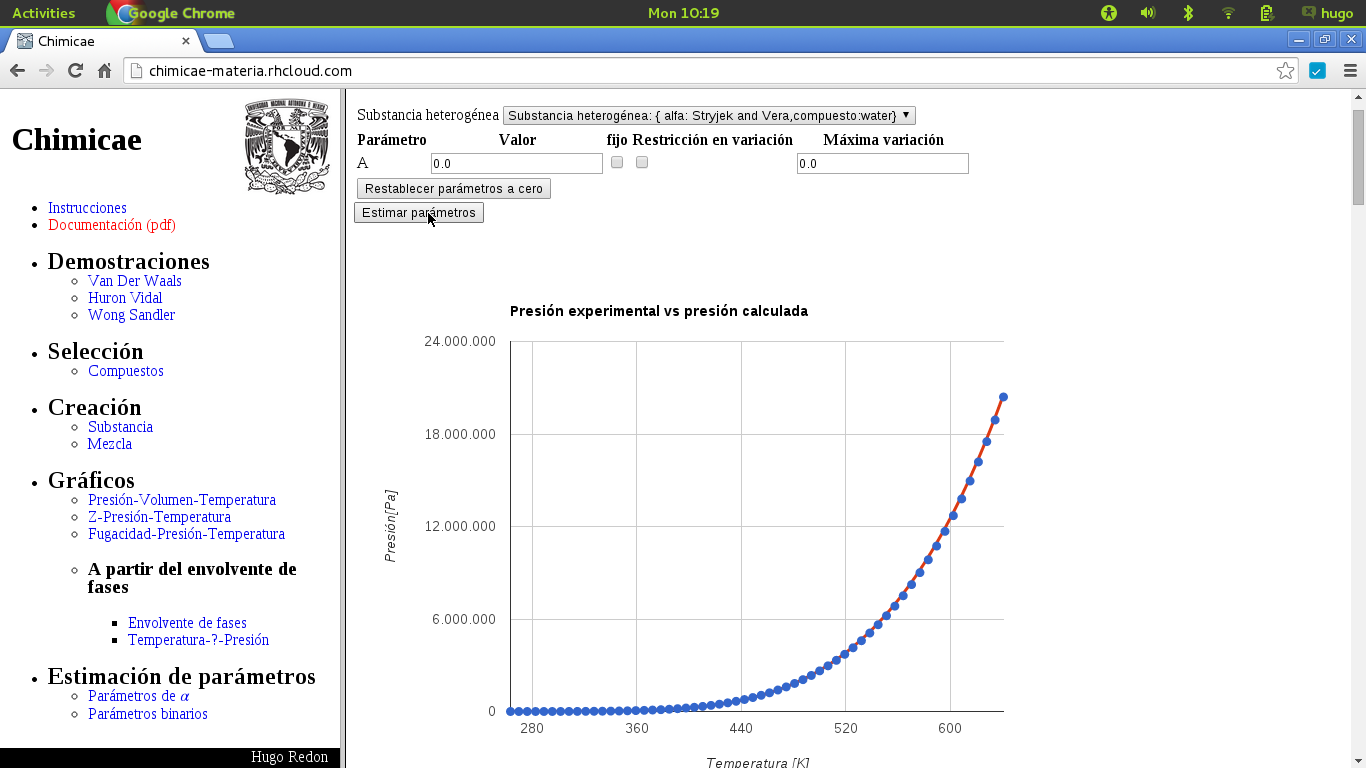
\includegraphics[scale=0.3]{waterAlphaOptPlot.png}
	\caption{Formulario para la estimación de parámetros de la expresión de $\alpha$}
	\label{fig:alphaOptim}
\end{figure}


\section{Estimación de parámetros binarios de las reglas de mezclado}\label{sec:webBinaryOptim}
	En la sección de `Estimación de parámetros' - `Parámetros binarios' podemos seleccionar una de las mezclas creadas previamente y estimar los parámetros de la regla de mezclado con datos que deberán ser agregados previamente a la página de internet.

	De manera semejante a la sección anterior, en la página se realiza una comparación de los datos experimentales con el modelo, se muestra una gráfica del error relativo y la historia de la convergencia.

	Una imagen del formulario se presenta en la figura \ref{fig:binaryOptim}
\begin{figure}[H]
	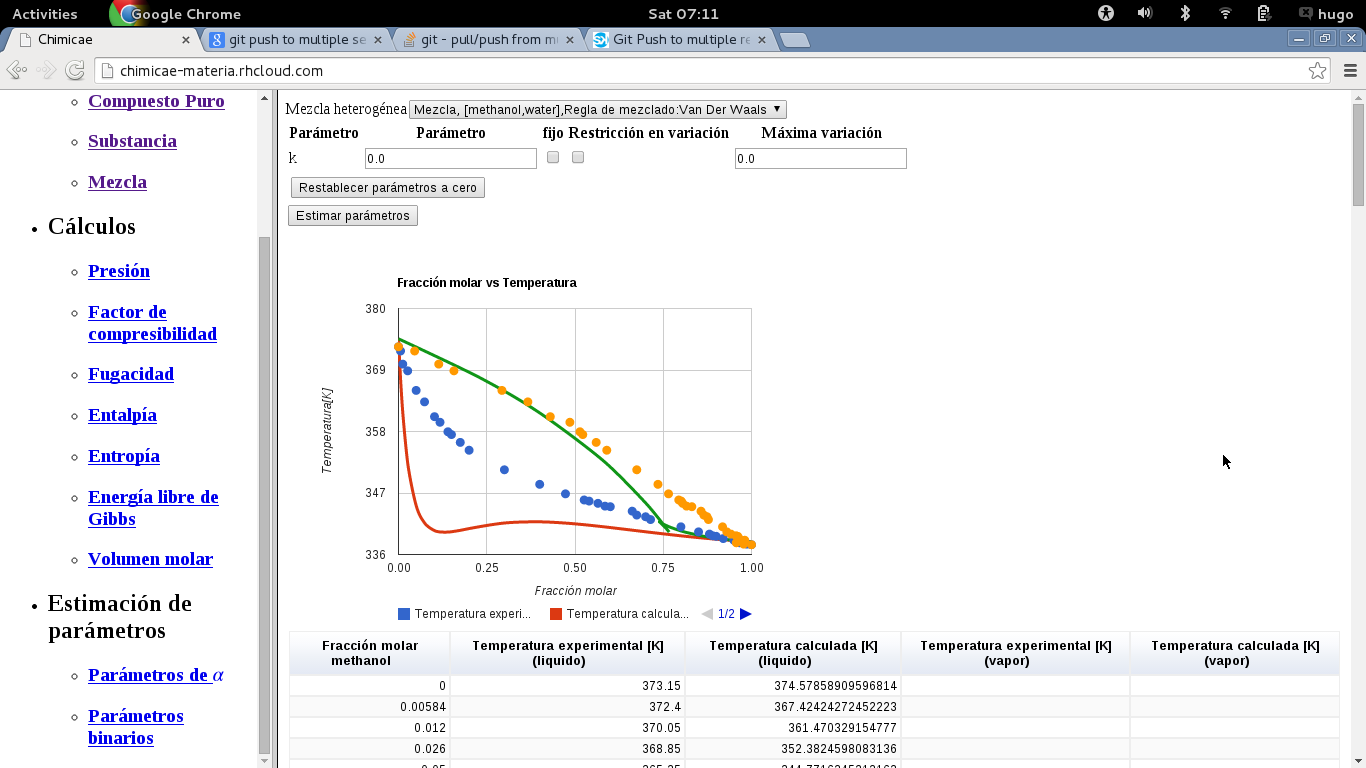
\includegraphics[scale=0.3]{waterMethanolBinaryOptPlot.png}
	\caption{Formulario para la estimación de parámetros de la regla de mezclado de Van Der Waals}
	\label{fig:binaryOptim}
\end{figure}

	\chapter{Extender o corregir la librería Materia}\label{chap:libraryExtension}

	Para colaborar con el proyecto \Materia y agregar nuevas clases a la biblioteca es necesario seguir los pasos del apéndice \ref{chap:github} para descargar el código fuente desde GitHub.	
	
 	En este capítulo se mostrará como crear nuevas:

 	\begin{itemize}\itemsep0ex
 		\item{Expresiones de $\alpha$}
 		\item{Reglas de Mezclado}
 		\item{Modelos de actividad} 		
 		\item{Ecuaciones de capacidad calorífica} 		
 	\end{itemize}

 
 	\section{Creación de nuevas expresiones de $\alpha$}\label{sec:newAlphaExpressions}

 	La estructura de una expresión de $\alpha$ depende de dos métodos fundamentales: 

 		\begin{itemize}\itemsep0ex
 			\item El cálculo de la expresión para una temperatura y un compuesto puro.
 			\item El cálculo de la derivada de la expresión con respecto a la temperatura, en específico la librería necesita el cálculo de la siguiente expresión.

 			\begin{equation}
 				\frac{T \partial \alpha}{\alpha \partial T}
 			\end{equation}
 		\end{itemize}

 	Para asegurar el funcionamiento de la estimación de los parámetros de la ecuación se necesitan adicionalmente los métodos:
 		\begin{itemize}\itemsep0ex
 			\item `getParameter'
 			\item `setParámeter'
 			\item `numberOfParameters'
 		\end{itemize}

	.

	Todos los métodos mencionados anteriormente se declaran en la clase abstracta `Alpha' y necesitan ser definidos en la nueva clases. 

	La nueva clase deberá heredar a la clase abstracta `Alpha', y definir los métodos abstractos de ella. 

	Los ambientes de desarrollo como Netbeans o Eclipse pueden generar lo necesario para definir una nueva expresión de $\alpha$. El código \ref{lst:newAlphaCode} muestra la nueva clase `NewAlphaExpresion' que hereda a la clase `Alpha' y define los métodos abstractos.


	\begin{lstlisting}[caption={Esqueleto para la creación de una nueva expresión de $\alpha$ para la librería materia, generado con el ambiente de desarrollo Eclipse},label={lst:newAlphaCode}]
import termo.component.Compound;
import termo.eos.alpha.Alpha;

public class NewAlphaExpresion extends Alpha {

	@Override
	public double TempOverAlphaTimesDerivativeAlphaRespectTemperature(
			double arg0, Compound arg1) {
		// TODO Auto-generated method stub
		return 0;
	}

	@Override
	public double alpha(double arg0, Compound arg1) {
		// TODO Auto-generated method stub
		return 0;
	}

	@Override
	public double getParameter(Compound arg0, int arg1) {
		// TODO Auto-generated method stub
		return 0;
	}

	@Override
	public String getParameterName(int arg0) {
		// TODO Auto-generated method stub
		return null;
	}

	@Override
	public int numberOfParameters() {
		// TODO Auto-generated method stub
		return 0;
	}

	@Override
	public void setParameter(double arg0, Compound arg1, int arg2) {
		// TODO Auto-generated method stub

	}

}

	\end{lstlisting}

	Existen expresiones de $\alpha$ que se definen para temperaturas debajo de la temperatura crítica y la ecuación cambia cuando la temperatura es mayor a la crítica, para tales casos existe la clase `TwoEquationsAlpha' que define los mismos métodos que la clase abstracta `Alpha' pero condiciona la salida de los métodos según las condiciones de temperatura. 

	El código \ref{lst:twoAlphaExample} utiliza dos expresiones de $\alpha$ y las pone dentro de un objeto `TwoEquationsAlpha' esta ecuación es la expresión de Mathias.

\begin{lstlisting}[caption={Creación de una expresión de $\alpha$ con cambio de ecuación según la temperatura del sistema},label={lst:twoAlphaExample}]
	TwoEquationsAlphaExpression mathias = new TwoEquationsAlphaExpression();    
	mathias.setName(AlphaNames.Mathias);
	CommonAlphaEquation mathiasBelow = new MathiasAlpha();
    
	MathiasAboveTcAlphaEquation mathiasAbove = new MathiasAboveTcAlphaEquation(mathiasBelow);
    
	mathias.setAlphaBelowTc(mathiasBelow);
	mathias.setAlphaAboveTc(mathiasAbove);
	return mathias;     
\end{lstlisting}

\section{Creación de nuevas reglas de mezclado}\label{sec:newMixingRules}
	
	Los métodos fundamentales de las reglas de mezclado son :

	\begin{itemize}
		\item El cálculo del parámetro a de la ecuación cúbica.
		\item El cálculo del parámetro b de la ecuación cúbica.
		\item La derivada del parámetro a con respecto al número de moles de un compuesto i, en específico se necesita el cálculo de la expresión: 
		\begin{equation}
			\frac{1\partial a N^2}{N \partial N_i}
		\end{equation}
		\item La derivada del parámetro a con respecto a la temperatura, en específico se necesita el cálculo de la expresión: 
		\begin{equation}
			T \frac{\partial a}{\partial T}
		\end{equation}
	\end{itemize}

	Además para el correcto funcionamiento de la estimación de parámetros se necesitan los métodos: 
	\begin{itemize}
		\item `getParameter'
		\item `setParameter'
		\item `numberOfParámeters'
	\end{itemize}

	La diferencia de los métodos `get' y `set' para los parámetros de las expresiones de $\alpha$ y las reglas de mezclado son los argumentos que reciben, ya que para una regla de mezclado son necesarios dos compuestos como argumentos y para la expresión de $\alpha$ no.

	El código \ref{lst:newMixingRule} muestra la clase generada por Eclipse con los métodos necesarios para crear una nueva regla de mezclado.

	\begin{lstlisting}[caption={Esqueleto para la creación de una nueva regla de mezclado},label={lst:newMixingRule}]

import termo.binaryParameter.InteractionParameter;
import termo.component.Compound;
import termo.eos.mixingRule.MixingRule;
import termo.matter.Mixture;
import termo.matter.Substance;

public class NewMixingRule extends MixingRule {

	@Override
	public double a(Mixture arg0) {
		// TODO Auto-generated method stub
		return 0;
	}

	@Override
	public double b(Mixture arg0) {
		// TODO Auto-generated method stub
		return 0;
	}

	@Override
	public double getParameter(Compound arg0, Compound arg1,
			InteractionParameter arg2, int arg3) {
		// TODO Auto-generated method stub
		return 0;
	}

	@Override
	public int numberOfParameters() {
		// TODO Auto-generated method stub
		return 0;
	}

	@Override
	public double oneOverNParcial_aN2RespectN(Substance arg0, Mixture arg1) {
		// TODO Auto-generated method stub
		return 0;
	}

	@Override
	public void setParameter(double arg0, Compound arg1, Compound arg2,
			InteractionParameter arg3, int arg4) {
		// TODO Auto-generated method stub

	}

	@Override
	public double temperatureParcial_a(Mixture arg0) {
		// TODO Auto-generated method stub
		return 0;
	}

}

	\end{lstlisting}

\section{Creación de nuevos modelos de Actividad}\label{sec:newActivityModels}

	Para las reglas de mezclado basadas en la energía libre de Gibbs son necesarios los modelos de actividad, y en la librería Materia es posible crear nuevos modelos.

	La clase abstracta `ActivityModel' declara los métodos necesarios para los modelos de actividad.

	\begin{itemize}
		\item El cálculo del coeficiente de actividad.
		\item El cálculo de la energía libre de Gibbs.
		\item El cálculo de la derivada de la energía libre de Gibbs con respecto a la temperatura.
	\end{itemize}

	Los modelos de actividad también tienen parámetros que se pueden estimar, pero para los modelos actualmente creados se ha utilizado la expresión de $\tau$ :

	\begin{equation}
		\tau = \frac{a_{ij} + b_{ij} T}{R T}
	\end{equation}

	y se han creado los métodos `get' y `set' parámeter para estos parámetros. Por lo cual si el modelo de actividad contiene mas parámetros que pueden ser estimados se deberán sobreescribir los métodos `get' y `set' para incluir los demás parámetros.

	El código \ref{lst:newActivityModel} muestra la clase generada por Eclipse para la creación de un nuevo modelo de actividad.

	\begin{lstlisting}[caption={Esqueleto de clase para la creación de un nuevo modelo de actividad},label={lst:newActivityModel}]

import java.util.ArrayList;
import java.util.HashMap;

import termo.activityModel.ActivityModel;
import termo.binaryParameter.ActivityModelBinaryParameter;
import termo.component.Compound;
import termo.matter.Mixture;
import termo.matter.Substance;

public class NewActivityModel extends ActivityModel {

	@Override
	public double activityCoefficient(Substance arg0, Mixture arg1) {
		// TODO Auto-generated method stub
		return 0;
	}

	@Override
	public double excessGibbsEnergy(Mixture arg0) {
		// TODO Auto-generated method stub
		return 0;
	}

	@Override
	public double parcialExcessGibbsRespectTemperature(
			ArrayList<Compound> arg0, HashMap<Compound, Double> arg1,
			ActivityModelBinaryParameter arg2, double arg3) {
		// TODO Auto-generated method stub
		return 0;
	}

}
	\end{lstlisting}


\section{Creación de nuevas ecuaciones de capacidad calorífica}\label{sec:newCpEquation}

	A diferencia de los objetos anteriores la capacidad calorífica se define como una interfaz `CpEquation', y para crear una nueva ecuación no es necesario heredar de ella, se debe implementar.


	El código \ref{lst:newCpEquation} muestra la implementación generada por eclipse para una nueva ecuación de capacidad calorífica.

	\begin{lstlisting}[caption={Esqueleto para crear una nueva ecuación de capacidad calorífica}, label={lst:newCpEquation}]

import termo.cp.CpEquation;

public class NewCpEquation implements CpEquation {

	public double Enthalpy(double arg0, double arg1, double arg2) {
		// TODO Auto-generated method stub
		return 0;
	}

	public double cp(double arg0) {
		// TODO Auto-generated method stub
		return 0;
	}

	public String getMathEquation() {
		// TODO Auto-generated method stub
		return null;
	}

	public double idealGasEntropy(double arg0, double arg1, double arg2,
			double arg3, double arg4) {
		// TODO Auto-generated method stub
		return 0;
	}

}
	\end{lstlisting}


	%\chapter{Diagramas ternarios}

\newcommand{\alphaOptim}[1] {

\begin{tabular}{c c}

\begin{tikzpicture}
	\begin{axis}
		\addplot[blue,only marks,mark size = 1pt]table[x=Temperature,y=experimentalPressure]{plotdata/ternaryDiagram/#1/afterOptim.dat};
		\addplot[red,thick]table[x=Temperature,y=calculatedPressure]{plotdata/ternaryDiagram/#1/afterOptim.dat};
	\end{axis}
\end{tikzpicture}
&
\begin{tikzpicture}
	\begin{axis}
		\addplot[blue,only marks,mark size = 1pt]table[x=Temperature,y=experimentalPressure]{plotdata/ternaryDiagram/#1/beforeOptim.dat};
		\addplot[red,thick]table[x=Temperature,y=calculatedPressure]{plotdata/ternaryDiagram/#1/beforeOptim.dat};
	\end{axis}
\end{tikzpicture}
\\
\begin{tikzpicture}
	\begin{axis}
		\addplot[blue,only marks,mark size = 1pt]table[x=Temperature,y=error]{plotdata/ternaryDiagram/#1/beforeOptim.dat};
		\addplot[red,only marks,mark size = 1pt]table[x=Temperature,y=error]{plotdata/ternaryDiagram/#1/afterOptim.dat};
	\end{axis}
\end{tikzpicture}
&
\begin{tikzpicture}
	\begin{axis}
		\addplot[only marks,mark size = 1pt]table[x=iteration,y=A]{plotdata/ternaryDiagram/#1/history.dat};
		\addplot[only marks,mark size = 1pt]table[x=iteration,y=B]{plotdata/ternaryDiagram/#1/history.dat};
		\addplot[only marks,mark size = 1pt]table[x=iteration,y=C]{plotdata/ternaryDiagram/#1/history.dat};
	
	\end{axis}
\end{tikzpicture}
\\
\begin{tikzpicture}
	\begin{axis}
		\addplot[red,only marks,mark size = 1pt]table[x=iteration,y=Error]{plotdata/ternaryDiagram/#1/history.dat};
	\end{axis}
\end{tikzpicture}
\end{tabular}
}


\newcommand{\binary}[1]{
\begin{tikzpicture}
	\begin{axis}
		\addplot[blue,only marks,mark size = 1pt]table[x=x1,y=pressure]{plotdata/ternaryDiagram/#1/beforeOptim.dat};
		\addplot[red,only marks,mark size = 1pt]table[x=y1,y=pressure]{plotdata/ternaryDiagram/#1/beforeOptim.dat};
		\addplot[green,thick]table[x=y1calc,y=calcpressure]{plotdata/ternaryDiagram/#1/beforeOptim.dat};
		\addplot[brown,thick]table[x=x1,y=calcpressure]{plotdata/ternaryDiagram/#1/beforeOptim.dat};

		\addplot[purple,thick]table[x=y1calc,y=calcpressure]{plotdata/ternaryDiagram/#1/afterOptim.dat};
		\addplot[black,thick]table[x=x1,y=calcpressure]{plotdata/ternaryDiagram/#1/afterOptim.dat};
	\end{axis}
\end{tikzpicture}

}

\alphaOptim{ethylene}
\alphaOptim{water}
\alphaOptim{ethanol}


binary



\binary{ethylenewater}



\begin{tikzpicture}
\begin{ternaryaxis}[xlabel=Agua,
ylabel=Etileno,
zlabel=Etanol]
\addplot3[only marks,blue] table[x=x1,y=x2,z=x3]{plotdata/ternaryDiagram/graph.dat};
\addplot3[only marks,red] table[x=y1,y=y2,z=y3]{plotdata/ternaryDiagram/graph.dat};
\end{ternaryaxis}
\end{tikzpicture}

	\chapter{Conclusiones}\label{chap:conclusions}

	Durante este proyecto se ha creado una librería de clases en java que resuelven el equilibrio entre fases para substancias y mezclas multi-componentes, además se ha logrado incluir métodos de optimización de parámetros de la expresión de $\alpha$ para el cálculo del parámetro $a$ de la ecuación de estado cúbica y de parámetros de interacción binaria de las reglas de mezclado y modelos de coeficientes de actividad para los casos que apliquen.

	La biblioteca permite representar las propiedades de las sustancias para poder realizar cálculos de interés en la ingeniería química.

	Las ecuaciones de estado incluidas en este proyecto se muestran en la tabla \ref{tab:cubics}, las expresiones de $\alpha$ se muestran en la tabla \ref{tab:alphas}, las reglas de mezclado se muestran en la tabla \ref{tab:mixingrules} y los modelos de coeficientes de actividad se muestran en la tabla \ref{tab:activitymodels}.

	La estructura de la librería y las herramientas utilizadas para su creación permiten la participación de un gran grupo de programadores para la realización de programas mas complejos.

	La creación de una página de internet para mostrar las principales funciones de la librería es un gran ejemplo del alcance de la librería.



	\appendix
	\chapter{Ejemplo de uso con Netbeans} \label{}



	\section{Requisitos}

	\begin{enumerate}

	\item Necesitamos tener instalado kit de desarrollo Jdk de java que se puede descargar desde la página (http://www.oracle.com/technetwork/java/javase/downloads/).

	\item Necesitamos tener instalado el ambiente de desarrollo Netbeans que se puede descargar de la página (https://netbeans.org/downloads/).
	\end{enumerate}

	\section{Manualmente}\label{sec:manualInstall}
		Descargar el archivo .jar y agregarlo al folder /lib de la aplicación
		\begin{enumerate}
			\item Desde la página oficial de EQ PRO(ingenieria-eqpro.rhcloud.com) se puede descargar el archivo jar.

			\item Crear un nuevo proyecto desde Netbeans.

			\begin{center}
			  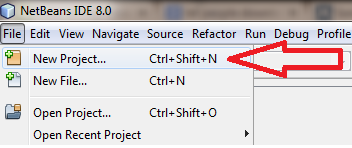
\includegraphics[scale=0.7]{new-proyect.png}
			\end{center}

			\item Elegir el tipo de aplicación java.application 
			\begin{center}
			  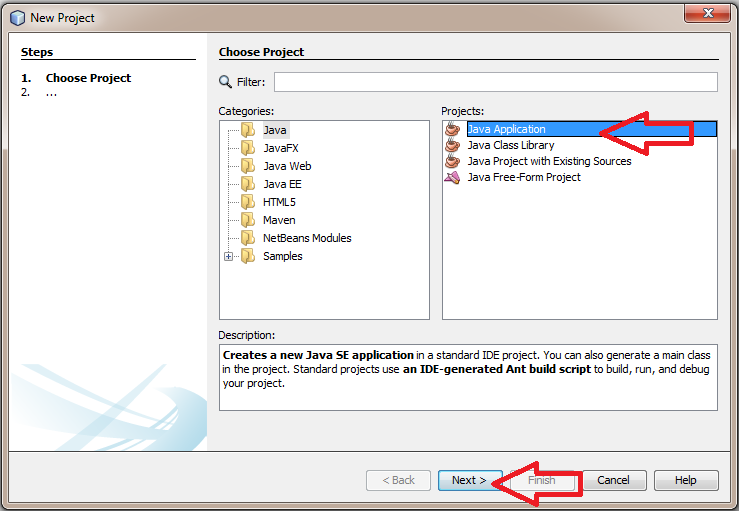
\includegraphics[scale=0.7]{application-type.png} 
			\end{center}
			\item Asignar el nombre del proyecto 
			\begin{center}
			  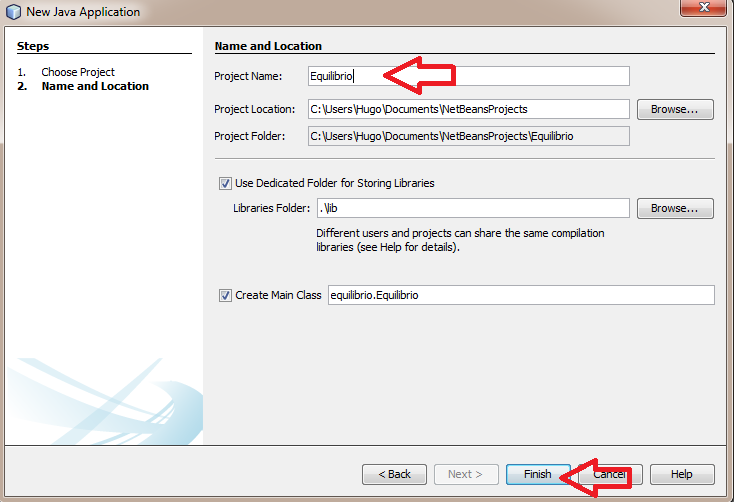
\includegraphics[scale=0.7]{proyect-name.png} 
			\end{center}
			\item En la pestaña proyectos de netbeans, con click derecho en la carpeta “Libraries” elegir la opción “Agregar jar/Folder “.
			\begin{center}
			  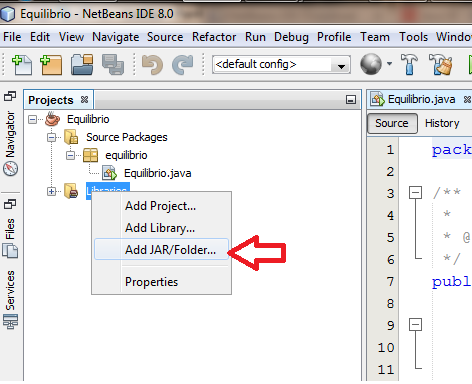
\includegraphics[scale=0.7]{add-jar.png} 
			\end{center}


			 \item Navegar entonces hasta la ruta donde se descargo el archivo jar. 

			\begin{center}
			  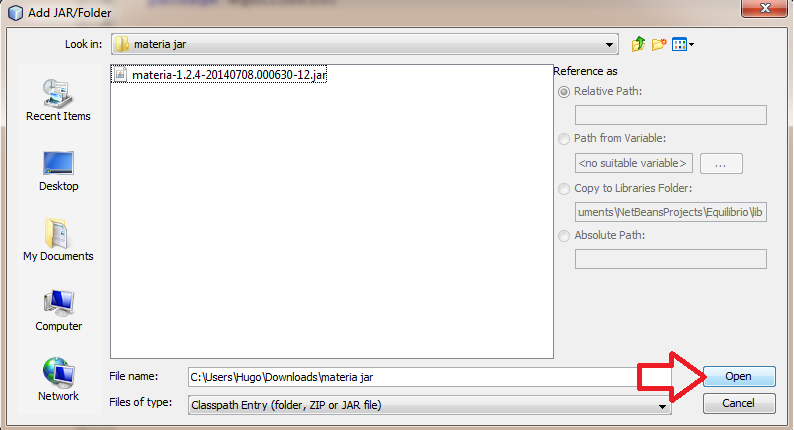
\includegraphics[scale=0.7]{select-materia-jar.png} 
			\end{center}

			Se puede ver entonces la librería agregada al proyecto.

			\begin{center}
			  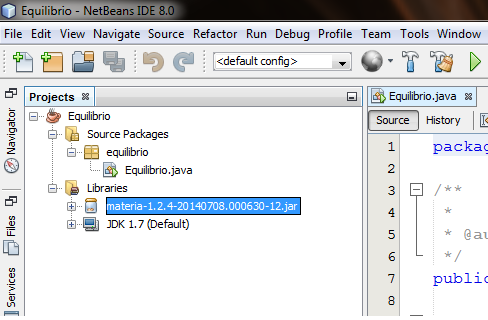
\includegraphics[scale=0.7]{library-added.png} 
			\end{center}
		\end{enumerate}

	\section{Maven}

		Desde maven utilizando el archivo pom.xml.
		    Crear nuevo proyecto :new proyect
		     Elegir la categoría ->Maven ->Java Applicationmaven java app
		    Elegir nombre del proyecto y dar click en finalizar.maven name
		    Podemos ver en la carpeta del proyecto la siguiente estructura
		\begin{verbatim}
		    Maven_Equilibrio
		    |-- pom.xml
		    `-- src
		        -- main
		           `-- java
		               `-- hugo
		                   `-- ejemplos
		                       `-- maven_equilibrio
		\end{verbatim}
		Abrimos el archivo pom.xml y agregamos las siguientes etiquetas


		\begin{lstlisting}[language=XML,morekeywords={repositories,
    repository,id,name,url,groupId,artifactId,dependencies,dependency}]
<dependencies>
  <dependency>
   <groupId>com.github.hugoredon</groupId>
   <artifactId>materia</artifactId>
   <version>1</version>
  </dependency>
</dependencies>
\end{lstlisting}


		5- Inmediatamente se ve agregada la dependencia Materia, cuando el proyecto se compile, se descargará el archivo jar automáticamente.

		maven materia added

		6.  Crear una clase java en cualquier paquete dentro de Source packages.maven create java class

		Escribimos dentro de esta clase el mismo código que en la entrada anterior.

	\section{Código}
		\begin{lstlisting}
			
		public class Equilibrio {
		 public static void main(String[] args) {
		 Compound agua = new Compound("agua");
		 agua.setCriticalTemperature(647.3);
		 agua.setCriticalPressure(2.212E7);
		 agua.setAcentricFactor(0.344861);
		 
		 Cubic cubicEquationOfState = EquationOfStateFactory.pengRobinsonBase();
		 Alpha alphaExpression = AlphaFactory.getStryjekAndVeraExpression();
		 
		 HeterogeneousSubstance substance =
		 new HeterogeneousSubstance(cubicEquationOfState, alphaExpression, agua);
		 double pressure = 101325;
		 substance.setPressure(pressure);
		 substance.bubbleTemperature();
		 double temperature = substance.getTemperature();
		 
		 System.out.println("(Presi|ó|n "+pressure+" [Pa])Temperatura de burbuja: " + temperature + "[K]");
		 }
		}

		\end{lstlisting}
		Ejecutamos el código y el resultado es:

		(Presión 101325.0 [Pa])Temperatura de burbuja: 374.5312063949659[K]%Ejemplo de uso de la libreria con netbeans instalación manual e instalación con Maven
	\chapter{Uso de GitHub, Git y JUnit para modificar la librería Materia}\label{chap:github}

Para mayor información sobre la participación en proyectos de GitHub, se recomienda la lectura de las guias:

\begin{itemize}\itemsep0ex
	\item Hola Mundo en GitHub, \url{https://guides.github.com/activities/hello-world/}
	\item Copias personales `Forking', \url{https://guides.github.com/activities/forking/}
	\item Seguimiento de errores y mejoras, \url{https://guides.github.com/features/issues/}
	\item Contribuyendo a proyectos Open-Source, \url{https://guides.github.com/activities/contributing-to-open-source/}
\end{itemize}

Para mayor información sobre Git se recomienda leer la documentación de la página oficial:
\begin{itemize}\itemsep0ex
	\item \url{http://git-scm.com/}
\end{itemize}

Para mayor infomación sobre JUnit se recomienda visitar la página:
\begin{itemize}\itemsep0ex
	\item \url{http://junit.org/}
\end{itemize}

	A continuación se listan brevemente los pasos necesarios para obtener y contribuir a la bliblioteca de clases Materia, es necesario tener una cuenta en GitHub y tener instalados \href{http://git-scm.com/}{Git} y \href{http://maven.apache.org/download.cgi}{Maven} en la computadora.

	\begin{enumerate}\itemsep0ex
		\item Encuentra algo en qué trabajar. Ya sea que encuentres un error en la biblioteca, quieras realizar una mejora o crear una nueva función primero debes estar seguro de lo que quieres hacer. 

		\item Archiva el asunto. Para evitar que dos personas trabajen en el mismo error, o intenten crear funciones semejantes es necesario llevar un registro de lo que se esta realizando en la biblioteca, para ello existe la sección `issues' en la página de GitHub de la biblioteca Materia \url{https://github.com/HugoRedon/Materia}. Ver la figura \ref{fig:issuesMateria}. Para mas información sobre como archivar asuntos en GitHub referirse a la guía de ayuda \url{https://guides.github.com/features/issues/}.

		\begin{figure}[!h]
			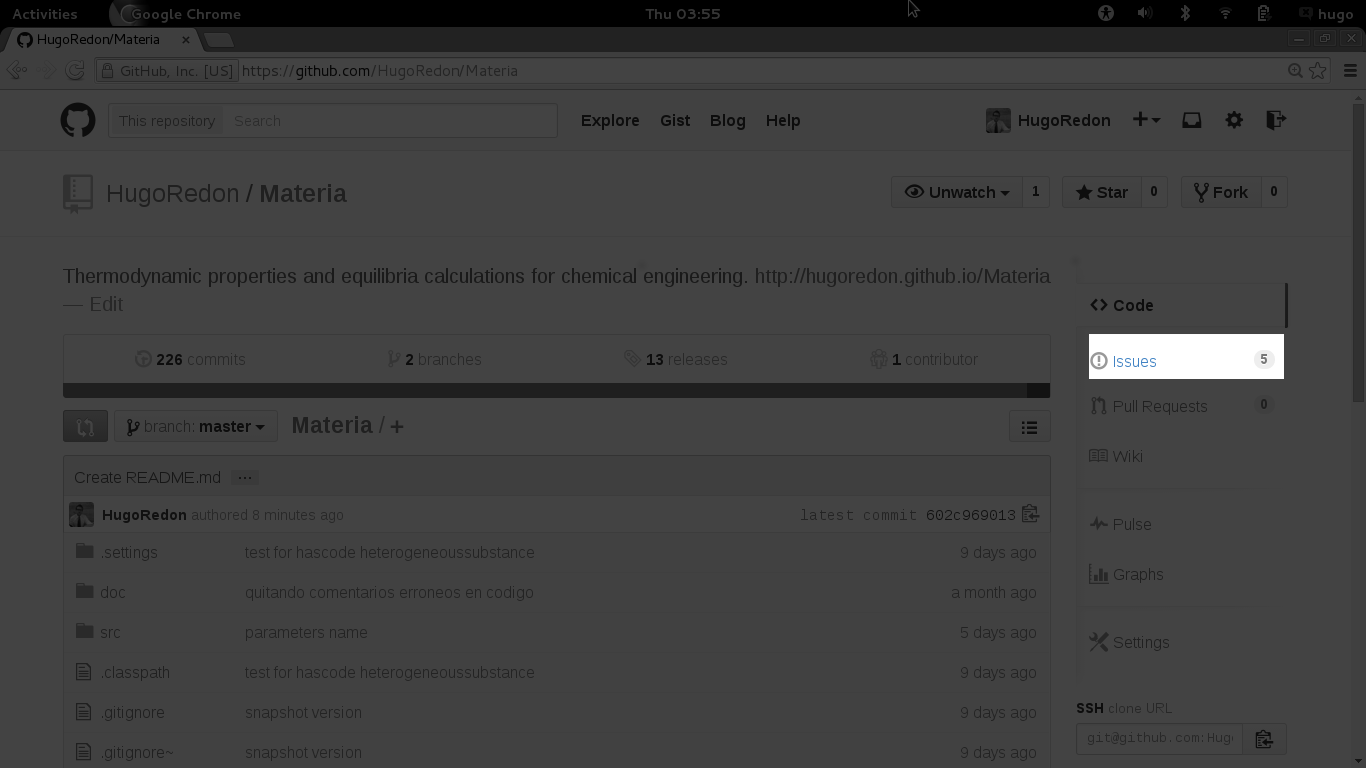
\includegraphics[scale=0.3]{materiaIssues.png}
			\caption{Página de GitHub de la biblioteca Materia, la sección resaltada permite archivar asuntos de error o mejoras en la biblioteca.}
			\label{fig:issuesMateria}
		\end{figure}

		\item Crea una copia personal de la biblioteca en tu cuenta de GitHub `Fork'. Para realizar una copia solo debes dirigirte a la página de GitHub del proyecto \href{https://github.com/HugoRedon/Materia}{Materia} y dar click en el boton `Fork', ver la figura \ref{fig:forkMateria}.

		\begin{figure}[!h]
			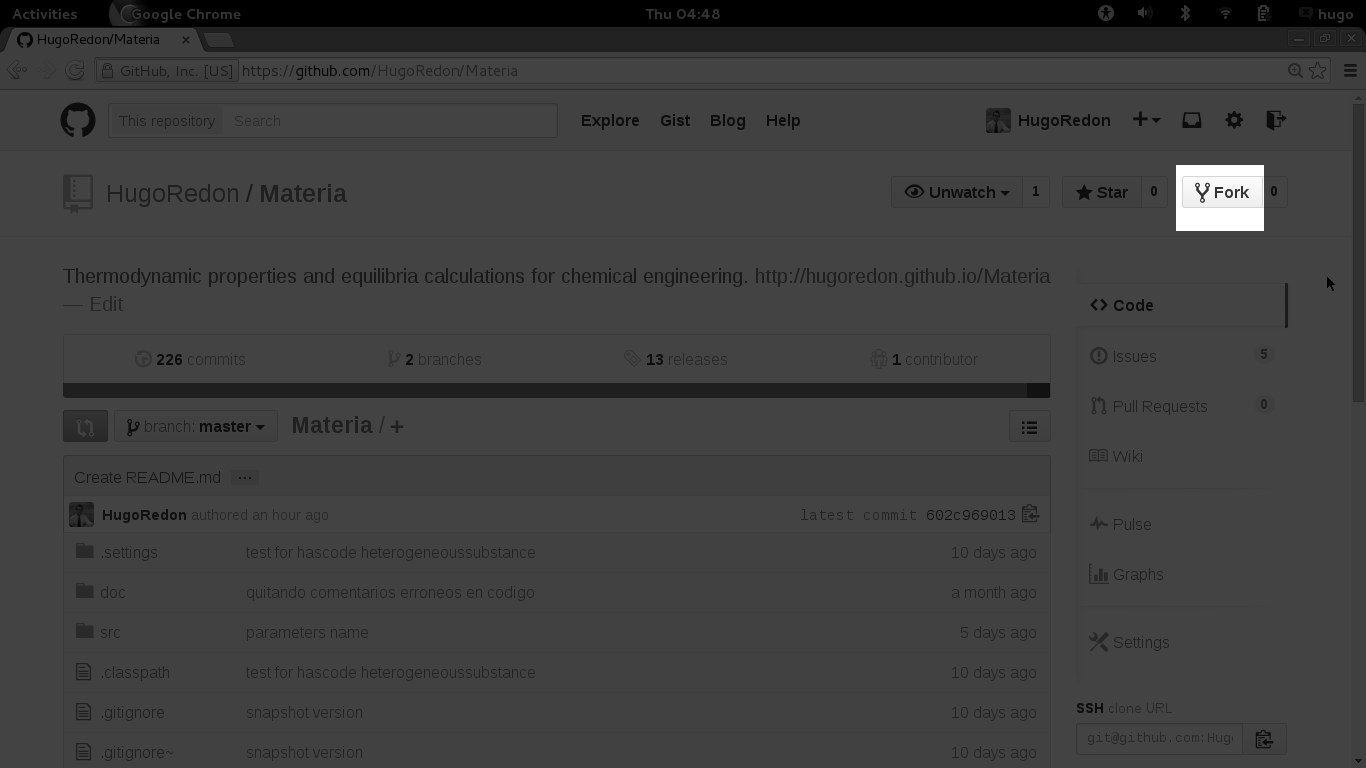
\includegraphics[scale=0.3]{forkMateria.png}
			\caption{Para realizar una copia personal de la biblioteca Materia solo se debe dar click en el boton `Fork'}
			\label{fig:forkMateria}
		\end{figure}

		\item Clona tu copia personal de la biblioteca Materia en tu computadora. 
			\begin{itemize}\itemsep0ex
				\item En github navega a tu copia personal del proyecto Materia
				\item En la barra derecha de la página, da click en el boton 
\includegraphics[scale=0.4]{clonebutton.png} para copiar la url del repositorio.
				\begin{figure}[!h]
					\centering
					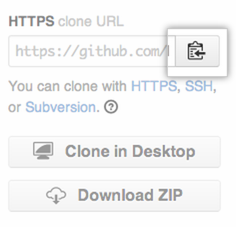
\includegraphics[scale=0.5]{cloneArea.png}.
				\end{figure}
				\item Abre una terminal (para usuarios de Mac y Linux) o linea de comando (usuarios de Windows).
				\item Escribe el comando  `git clone' y después pega la url del paso 2. El resultado debe ser algo semejante al código \ref{lst:cloneCommand}

\begin{lstlisting}[label={lst:cloneCommand},caption={Commando para clonar el repositorio de GitHub},language=bash]
	$ git clone https://github.com/<Nombre de usuario>/Materia
\end{lstlisting}

			\end{itemize}

		\item Crear la rama donde se realizarán los cambios. Para trabajar de forma segura se debe crear una rama donde se desarrollen las nuevas funciones o la corrección a la librería Materia. Esto se logra con el commando \ref{lst:newBranch}. El nombre de la nueva rama debe ser consistente con la tarea a realizar.
		\begin{lstlisting}[label={lst:newBranch},caption={Commando para crear una nueva rama en el repositorio.},language=bash]
			$ git checkout -b <nombre de la nueva rama>
		\end{lstlisting}

		\item Crear las pruebas necesarias que aseguren el funcionamiento del cambio que se desea realizar. El primer paso para resolver un problema es entender el problema. La creación de una prueba ayuda en el proceso de entendimiento del problema. Para ejecutar las pruebas se utiliza el commando de Maven que se muestra en el fragmento de código \ref{lst:mvnTest}. Las pruebas deberán ser creadas en el folder src/test/java dentro del paquete de la clase que se esté probando.

\begin{lstlisting}[caption={Para ejecutar las pruebas del proyecto},label={lst:mvnTest},language=bash]
	$ mvn test
\end{lstlisting}

		Dado que no se ha modificado aún el código, el resultado del comando anterior solo debería encontrar fallas en las pruebas nuevas agregadas.

		\item Escribir las nuevas funciones o las correcciones al código hasta conseguir el éxito en las pruebas. Una vez escritas las pruebas el objetivo del programador es modificar el código hasta que todas las pruebas del código pasen sin errores, es decir que la nueva prueba creada se ejecuta como se esperaba y que ninguna otra prueba ha sido alterada en el proceso.

		\item Agregar los cambios al repositorio local. Si durante el proceso de modificación se agregaron o eliminaron archivos podemos agregar los cambios al repositorio en la computadora mediante los commandos \ref{lst:addCommit}

\begin{lstlisting}[caption={Agregar los cambios al repositorio local.},label={lst:addCommit},language=bash]
	$ git add --all # Agregando los cambios 
	$ git commit -m "<Nota que explique los cambios realizados>" 
		#Archivando los cambios
\end{lstlisting}
		
		Es importante que la nota responda las siguientes preguntas o necesidades:
			\begin{itemize}\itemsep0ex
	 			\item ¿Qué cambios se hicieron al código?
	 			\item ¿Porque se realizaron los cambios al código? ó ¿Qué problema resuelven los cambios agregados? En caso de tener un número de asunto `issue' anotarlo en el comentario, y si este esta resuelto agregar el prefijo fix como se sugiere en la página: \url{https://help.github.com/articles/closing-issues-via-commit-messages}
	 			\item ¿Qué problemas surgieron durante el proceso?
	 			\item ¿Se encontraron otros problemas? si la repuesta es si, entonces listar cuales. De ser necesario crear los asuntos (paso 2) en la página principal de GitHub para ser tratados en el futuro.
		 	\end{itemize}

	 	\item Subir los cambios a la copia personal de GitHub. Hasta este punto solo el repositorio en la computadora contiene los cambios agregados. Para subir los cambios a internet se debe usar el comando \ref{lst:pushMateria}.

	 	\begin{lstlisting}[caption={Comando para agregar los cambios a la copia personal de GitHub},label={lst:pushMateria},language=bash]
	 		$ git push origin master 
	 	\end{lstlisting}

	 	Una vez ejecutado el comando los cambios deberán ser visibles en la página de GitHub, pero estos cambios existen solo en la copia personal.

	 	\item Compartir los cambios al proyecto original.Finalmente si se desea compartir los cambios realizado a la copia personal, es necesario realizar un `pull request', esto se logra dando click en el botón `compare \& pull request' ver la figura \ref{fig:pullRequestMateria}.

	 	\begin{figure}[!h]
	 		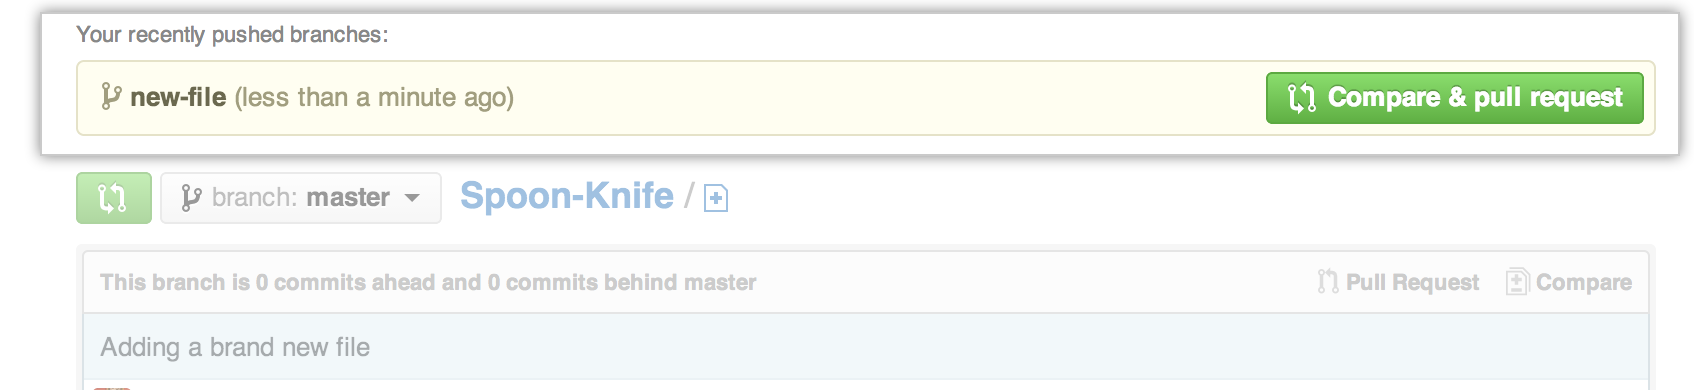
\includegraphics[scale=0.4]{recently_pushed_branch.png}
	 		 \caption{Sección para compartir los cambios al proyecto original.}
	 		 \label{fig:pullRequestMateria}
	 	\end{figure}

	 	Al dar click en el botón serás enviado a una página de discusión donde se debe escribir un título y una descripción sobre la petición para agregar los cambios. Finalmente si los cambios son aceptados habrás concluido tu participación al proyecto Materia y tu perfil de GitHub se habrá agregado a la lista de contribuidores del proyecto Materia.

	\end{enumerate}



	\chapter{Ecuaciones}



\begin{equation}\label{eq:pressure}
P = \frac{R T}{v-b} - \frac{a}{v^2 +u b v + w b^2 }
\end{equation}


\begin{itemize}\itemsep0ex
\item $P$ : presión en $[Pa]$.
\item $v$ : volumen molar en $[\frac{m^3}{kg}]$
\item $a$ : Es una medida de la atracción entre las partículas. $[\frac{m^5}{kg s}]$
\item $b$ : volumen excluido por un mol de partículas.$[\frac{m^3}{kg}]$
\item $u$ y $w$ : Son los parámetros diferentes para cada ecuación de estado, ver tabla \ref{tab:cubics}
\item $R$ : Constante universal de los gases ideales en $\frac{m^3 Pa}{kgmol K}$
\end{itemize}


\begin{equation}\label{eq:a}
	b_i = \Omega_b \frac{R T_{ci}}{p_{ci}} 
\end{equation}

\begin{equation}\label{eq:b}
 a_i = \Omega_a \frac{\left(R T_{ci}\right)^2}{p_{ci}} \alpha_i
\end{equation}


\begin{equation}\label{eq:z}
z= \frac{P V}{R T}
\end{equation}

\begin{equation}\label{eq:volume}
V = \frac{R T}{z P}
\end{equation}

\begin{equation}\label{eq:AB}
A=\frac{ap}{(RT)^2}
\qquad
B=\frac{bp}{RT}
\end{equation}

\begin{equation}
z^3-\left[1-(u-1)B\right]z^2+ \\ \left[A-uB-uB^2 +\\ wB^2\right]z-\left[AB+wB^2+wB^3\right]=0
\end{equation}


\subsubsection{Entalpía del gas ideal}
\begin{equation}\label{eq:idealgasenthalpy}
h^{\neq} = \sum_{i=1}^{nc} x_i \left[ h_i^{ref} + \int_{Tref}^{T} Cp_i^{\neq} \mathrm{d}T \right]
\end{equation}

\section{Entalpía}
\begin{equation}\label{eq:enthalpy}
h = h^{\neq} + \left[ \frac{T(\frac{\partial a}{\partial T}) - a}{b\sqrt{u²-4w} }\right] 
\ln\left[\frac{2v+b\left(u + \sqrt{u²-4w}\right)}{2v+b\left(u - \sqrt{u²-4w}\right)}\right]
+ pv - RT
\end{equation}

\begin{lstlisting}[label=some-code,caption=Some Code]
private  double calculateEnthalpy( double volume){
    double idealGasEnthalpy = calculateIdealGasEnthalpy();
    double a = calculate_a_cubicParameter();
    double b = calculate_b_cubicParameter();
    double L = cubicEquationOfState.calculateL(volume, b);
    double partial_aPartial_temperature = partial_aPartial_temperature( );
    
    return idealGasEnthalpy + ((partial_aPartial_temperature - a)/b) * L  + pressure * volume - Constants.R *temperature;
}
\end{lstlisting}	



\subsection{Entropía}
\begin{equation}
s = s^{\neq} + R\ln\left[\frac{z(v-b)}{v}\right] + \frac{\frac{\partial a}{\partial T}}{b \sqrt{u^2 - 4w}}
\ln\left[\frac{2v+b\left(u + \sqrt{u²-4w}\right)}{2v+b\left(u - \sqrt{u²-4w}\right)}\right]
\end{equation}
\begin{equation}
s^{\neq} = \sum_{i=1}^{nc} x_i\left[s_i^{ref} + \int_{Tref}^T \frac{Cp_i^{\neq}}{T} \mathrm{d}T 
- R\ln \left(\frac{p}{p_{ref}}\right)- R\ln{x_i}
\right]
\end{equation}


\begin{equation}\label{eq:gibbs}
g = h - T * s;
\end{equation}


\begin{multline}\label{eq:fugacity}
\ln\hat{\phi_i} = - \ln\left(\frac{v-b}{v}\right) 
+ (z-1)\left[\frac{1}{b}\frac{\partial bN}{\partial N_i}\right]
+ \frac{a}{RTb\sqrt{u^2-4w}}
\\
\left[\frac{1}{b}\frac{\partial bN}{\partial N_i}
- \frac{1}{aN}\frac{\partial aN²}{\partial N_i}\right]
\ln\left[\frac{2v+b\left(u + \sqrt{u²-4w}\right)}{2v+b\left(u - \sqrt{u²-4w}\right)}\right]
-\ln{z}
\end{multline}
	\subsection{Expresiones de $\alpha$}

	\subsubsection{Soave\cite{soave}}

\begin{gather}
	\alpha^{\nicefrac{1}{2}} = 1 + m \left(1-\sqrt{T_r}\right)\\
	m = 0.48508+1.55171\omega-0.15613\omega^2
\end{gather}
	\subsubsection{Peng and Robinson \cite{pengRobinson}}


\begin{gather}
	\alpha^{\nicefrac{1}{2}} = 1 + m \left(1-\sqrt{T_r}\right)\\
	m = 0.37464+1.54226\omega-0.2699\omega^2
\end{gather}
	\subsubsection{Mathias\cite{mathias} }
\begin{itemize}

\item{$T < T_C$}
\begin{gather}
	\alpha^{\nicefrac{1}{2}} = 1 + m \left(1-\sqrt{T_r}\right)- A\left(1-T_r\right)\left(0.7-T_r\right)
	\\
	m = 0.48508+1.55191\omega-0.15613\omega^2
\end{gather}

\item{$T > T_c$}
\begin{gather}
	\alpha = \exp{\left[ \left( \frac{c-1}{c} \right)  \left(  1- T_r^c  \right)  \right]}\\
	c = 1 + \frac{m}{2} + 0.3 A
\end{gather}

 \end{itemize}


	\subsubsection{Stryjek and Vera(PRSV)\cite{stryjekVeraPureCompounds} }
\begin{itemize}

\item{$T < T_C$}
\begin{gather}
	\alpha^{\nicefrac{1}{2}} = 1 + \kappa_0 \left(1-\sqrt{T_r}\right)- \kappa_1\left(1-T_r\right)\left(0.7-T_r\right)
	\\
	\kappa_0 = 0.378893+1.4897153\omega-0.17131848\omega^2+0.0196554\omega³
\end{gather}

\item{$T > T_c$}
\begin{equation}
	\alpha^{\nicefrac{1}{2}} = 1 + \kappa_0\left(1- \sqrt{T_r}\right)
\end{equation}

 \end{itemize}	
	\subsubsection{Adachi and Lu \cite{adachiLu}}

\begin{equation}
\alpha = A\cdot {10}^{B\left(1-T_r\right)}
\end{equation}
	\subsubsection{Soave \cite{soaveR}}

\begin{equation}\label{eq:soaveR}
\alpha= 1+\left(1-T_r\right)\left(A + \frac{B}{T_r}\right)
\end{equation}
	\subsubsection{Melhem, et al.\cite{melhem}}

\begin{equation}
\ln{\alpha}=A\left(1-T_r\right)+ B\left(1-\sqrt{T_r}\right)^2
\end{equation}
	\subsubsection{Androulakis,et al.\cite{androulakis}}

\begin{itemize}
\item{$T < T_C$}
\begin{equation}
 \alpha = 1 + A \left(1-T_r^{\nicefrac{2}{3}}\right) + B\left(1-T_r^{\nicefrac{2}{3}}\right)^2+ C\left(1-T_r^{\nicefrac{2}{3}}\right)^3
\end{equation}
\item{$T > T_c$}
\begin{equation}
\alpha = \mathrm{e}^{A\left(1-T_r^{\nicefrac{2}{3}}\right)}
\end{equation}
\end{itemize}
	\subsubsection{Mathias and Copeman. \cite{mathiasCopeman,michelsen}}

\begin{itemize}
\item{$T < T_c$}
\begin{equation}
\alpha^{\nicefrac{1}{2}} = 1 + A\left(1-\sqrt{T_r}\right) + B\left(1-\sqrt{T_r}\right)^2 + C\left(1-\sqrt{T_r}\right)^3
\end{equation}
\item{$T > T_c$}
\begin{equation}
\alpha^{\nicefrac{1}{2}} = 1 + A\left(1-\sqrt{T_r}\right)
\end{equation}
\footnote{La ecuación no se incluyó en el trabajo original de Mathias and Copeman\cite{mathiasCopeman}; esta expresión fue incorporada en el trabajo de Dahl and Michelsen \cite{michelsen}}
\end{itemize}
	\subsubsection{Yu and Lu\cite{yuLu}}

\begin{itemize}
\item{$T < T_c$}
\begin{equation}
 \log_{10}{\alpha} = \left(A+B T_r+ C T_r^2\right)\left(1-T_r\right)
\end{equation}
\item{$T > T_c$}
\begin{equation}
 \log_{10}{\alpha} = \left(A+B+C \right)\left(1-T_r\right)
\end{equation}
\end{itemize}
	\subsubsection{Stryjek and Vera\cite{stryjekVera}}

\begin{itemize}
\item{$T < T_c$}
\begin{gather}
\alpha^{\nicefrac{1}{2}} = 1 + \kappa\left(1-\sqrt{T_r}\right)\\
\kappa = m + \left[
		A+ B\left(C- T_r\right)\left(1-\sqrt{T_r}\right)
	\right]
	\left[
		\left(1+ \sqrt{T_r}\right)\left(0.7-T_r\right)
	\right]\\
m=0.378893 + 1.4897153 \omega - 0.17131848 \omega^2+ 0.0196554 \omega^3
\end{gather}
\item{$T > T_c$}
\begin{equation}
\alpha^{\nicefrac{1}{2}} = 1 + m\left(1-\sqrt{T_r}\right)
\end{equation}
\end{itemize}
	\subsubsection{Twu\cite{twuequation}}
\begin{equation}
	\alpha = T_r^{N\left(M-1\right)}\exp{\left(L\left(1-T_r^{N M}\right)\right)}
\end{equation}
	\subsubsection{Twu \cite{twuactivity}}
\begin{itemize}
\item{$T < T_c$}
\begin{gather}
\alpha = \alpha^{(0)} + \omega\left(\alpha^{(1)}-\alpha^{(0)}\right)\\
\text{Para}\qquad \alpha^{(0)}\notag\\
L= 0.196545\qquad M=0.906437\qquad N=1.26251\\
\text{Para}\qquad \alpha^{(1)}\notag\\
L=0.704001 \qquad M =0.790407 \qquad N=2.13076
\end{gather}
\item{$T > T_c$}
\begin{gather}
\alpha = \alpha^{(0)} + \omega\left(\alpha^{(1)}-\alpha^{(0)}\right)\\
\text{Para}\qquad \alpha^{(0)}\notag\\
L= 0.358826\qquad M=4.23478\qquad N=-0.2\\
\text{Para}\qquad \alpha^{(1)}\notag\\
L=0.0206444 \qquad M =1.22942 \qquad N=-8.0
\end{gather}
\end{itemize}
	\subsubsection{GCEOS (AspenHYSYS)}

\begin{gather}
\alpha^{\nicefrac{1}{2}} = 1 + \kappa \left(1 - \sqrt{T_r}\right)\\
\kappa = \kappa_0 + \left[ 
	\kappa_1 + \left(   \kappa_2 - \kappa_3 T_r   \right)
	\left(1 - T_r^{\kappa_4}\right) 
\right]
\left[
	\left(1 + \sqrt{T_r}\right)\left(0.7 - T_r\right)
\right]
T^{\kappa_5}\\
\kappa_0 = A + B \omega+ C \omega^2+ D \omega^3
\end{gather}




	\chapter{Algoritmos para el equilibrio Líquido-Vapor}\label{chap:algorithms}


%---------------------------saturationTemperature--------------------------------------------------------------
\begin{figure}[!h]
\begin{tikzpicture}[nodes={draw, fill=white,align=center},row sep=1.4cm,column sep=0.7cm] ]

\node(init){Inicio};
\node[below of=init,below] (lab)  {Lectura de \textbf{Datos} \\$P$};
\node[below of=lab,below = 0.4cm](estim){Estimado inicial de\\ la incognita\\$T$};
\node[below of=estim,below = 0.6](relations){Cálculo de la\\ razon de equilibrio\\
$K = \frac{ \hat{\phi}^L }{\hat{ \phi}^V}$};
\node[below of=relations,below = 0.6cm](error){Cálculo de la función Error\\$ E = \ln{K}$};

\node[below of=error,below = 0.6](criteria){$|E| \leq 1\cdot10^{-4}\quad \text{o} \quad  1\cdot 10^{-5}$};
\node[below of=criteria,below = 0.4](tempIncrement){Incrementar la temperatura\\$T^* = T + \Delta T$\\
$\Delta T = 0.1  \quad \text{o} \quad 1.0 K$};

\node[below of=tempIncrement,below = 0.4](relationsWithIncrement){Cálculo de las Razon\\ de Equilibrio con $T^*$
\\$K^* = \frac{ \hat{\phi}^L }{ \hat{\phi}^V}$};

\node[right of=criteria	,right=2.2cm](end){Fin};


\node[right of=tempIncrement, right=3cm](errorWithIncrement){Cálculo de la función Error \\ con $T^*$\\$ E^* = \ln{K^*}$};

\node[right of=relations, right = 3cm](newValues){Cálculo de la nueva estimación \\ de la \textbf{Incógnita}\\
\begin{minipage}{0.2\linewidth}
\begin{equation*}
T_{nueva} = \frac{TT^* \left(E^*-E\right)}{T^*E^*-TE}
\end{equation*}
\end{minipage}
};


\draw[-latex] (init)--(lab);
\draw[-latex] (lab)--(estim);
\draw[-latex] (estim)--(relations);
\draw[-latex] (relations)--(error);
\draw[-latex] (error)--(criteria);
\draw[-latex] (criteria)--node[fill=none,draw=none,above]{SI}(end);
\draw[-latex] (criteria)--node[fill=none,draw=none,left]{NO}(tempIncrement);
\draw[-latex] (tempIncrement)--(relationsWithIncrement);
\draw[-latex] (relationsWithIncrement)--(errorWithIncrement);
\draw[-latex] (errorWithIncrement)--(newValues);
\draw[-latex] (newValues)--(relations);

\end{tikzpicture}
\caption{Algoritmo de temperatura de saturación.}\label{fig:saturationtemperature}
\end{figure}










\begin{figure}[!h]
\begin{tikzpicture}[nodes={draw, fill=white,align=center},row sep=1.4cm,column sep=0.7cm] ]

\node(init){Inicio};
\node[below of=init,below] (lab)  {Lectura de \textbf{Datos} \\$P$};
\node[below of=lab,below = 0.4cm](estim){Estimado inicial de\\ la incognita\\$T=300 K$};
\node[below of=estim,below = 0.6](relations){Cálculo de la presión de vapor según\\ la ecuación del  factor acéntrico con $T$ \\\\
$ P\degree= P_c 10^{\displaystyle\left[\left(-\frac{7}{3}\right) \left(1+\omega \right)  \left(\left(\frac{T_c}{T}\right) - 1 \right) \right]}$};
\node[below of=relations,below = 1.1cm](error){Cálculo de la función Error\\$ E = \ln{\displaystyle\frac{P\degree}{P}}$};

\node[below of=error,below = 0.6](criteria){$|E| \leq 1\cdot10^{-4}\quad \text{o} \quad  1\cdot 10^{-5}$};
\node[below of=criteria,below = 0.4](tempIncrement){Incrementar la temperatura\\$T^* = T + \Delta T$\\
$\Delta T = 0.1  \quad \text{o} \quad 1.0 K$};

\node[below of=tempIncrement,below = 0.4](relationsWithIncrement){Cálculo de la presión de vapor según\\ la ecuación del factor acéntrico con $T^*$ \\\\
${P\degree}^*= P_c 10^{\displaystyle\left[\left(-\frac{7}{3}\right) \left(1+\omega \right)  \left(\left(\frac{T_c}{T^*}\right) - 1 \right) \right]}$};

\node[right of=criteria	,right=2.2cm](end){Fin};


\node[right of=tempIncrement, right=3cm](errorWithIncrement){Cálculo de la función Error\\$ E^* = \ln{\displaystyle\frac{{P\degree}^*}{P}}$};

\node[right of=relations, right = 3.5cm](newValues){Cálculo de la nueva estimación \\ de la \textbf{Incógnita}\\
\begin{minipage}{0.2\linewidth}
\begin{equation*}
T_{nueva} = \frac{TT^* \left(E^*-E\right)}{T^*E^*-TE}
\end{equation*}
\end{minipage}
};


\draw[-latex] (init)--(lab);
\draw[-latex] (lab)--(estim);
\draw[-latex] (estim)--(relations);
\draw[-latex] (relations)--(error);
\draw[-latex] (error)--(criteria);
\draw[-latex] (criteria)--node[fill=none,draw=none,above]{SI}(end);
\draw[-latex] (criteria)--node[fill=none,draw=none,left]{NO}(tempIncrement);
\draw[-latex] (tempIncrement)--(relationsWithIncrement);
\draw[-latex] (relationsWithIncrement)--(errorWithIncrement);
\draw[-latex] (errorWithIncrement)--(newValues);
\draw[-latex] (newValues)--(relations);

\end{tikzpicture}
\caption{Algoritmo de estimación de temperatura de saturación usando la ecuación del factor acéntrico.}
\label{fig:temperatureEstimate}
\end{figure}


%------------------------saturationPressure------------------------------------------------------------------------------------------------------------------


\begin{figure}
	\begin{tikzpicture}[nodes={draw, fill=white,align=center},row sep=0.3cm,column sep=0.5cm] ]

	\node(init){Inicio};
	\node[below of=init,below] (lab)  {Lectura de \textbf{Datos} \\$T$};
	\node[below of=lab,below=0.2cm](estim){Estimado inicial de\\ la incognita\\$P$};
	\node[below of=estim,below=0.6cm](relations){Cálculo de la\\ razon de equilibrio\\
	$K = \frac{ \hat{\phi}^L }{\hat{ \phi}^V}$};
	\node[below of=relations,below = 0.6cm](error){Cálculo de la función Error\\$ E = {K}-1 $};

	\node[below of=error,below=0.6cm](criteria){$|E| \leq 1\cdot10^{-4}\quad \text{o} \quad  1\cdot 10^{-5}$};
	\node[below of=criteria,below=0.4cm](pressureIncrement){Incrementar la presión\\$P^* = P + \Delta P$\\
	$\Delta P = 0.001  \quad \text{o} \quad 0.0001 K$};

	\node[below of=pressureIncrement,below=0.4cm](relationsWithIncrement){Cálculo de la Razon\\ de Equilibrio con $P^*$
	\\$K^* = \frac{ \hat{\phi}^L }{ \hat{\phi}^V}$};

	\node[right of=criteria	,right=2.2cm](end){Fin};


	\node[right of=pressureIncrement, right=3cm](errorWithIncrement){Cálculo de la función Error \\ con $P^*$\\$ E^* = K^* -1 $};

	\node[right of=relations, right = 3cm](newValues){Cálculo de la nueva estimacion \\ de la \textbf{Incógnita}\\
	\begin{minipage}{0.2\linewidth}
	\begin{equation*}
	T_{nueva} = \frac{P P^* \left(E^*-E\right)}{P^*E^*-P E}
	\end{equation*} 
	\end{minipage}
	};


	\draw[-latex] (init)--(lab);
	\draw[-latex] (lab)--(estim);
	\draw[-latex] (estim)--(relations);
	\draw[-latex] (relations)--(error);
	\draw[-latex] (error)--(criteria);
	\draw[-latex] (criteria)--node[fill=none,draw=none,above]{SI}(end);
	\draw[-latex] (criteria)--node[fill=none,draw=none,left]{NO}(pressureIncrement);
	\draw[-latex] (pressureIncrement)--(relationsWithIncrement);
	\draw[-latex] (relationsWithIncrement)--(errorWithIncrement);
	\draw[-latex] (errorWithIncrement)--(newValues);
	\draw[-latex] (newValues)--(relations);

	\end{tikzpicture}
	\caption{Algoritmo para el cálculo de presión de saturación.}\label{fig:saturationpressure}
\end{figure}

%-----------------------------------------bubbleTemp---------------------------------------------

\begin{figure}[!h]
	\begin{tikzpicture}[nodes={draw, fill=white,align=center},row sep=1.4cm,column sep=0.7cm] ]

	\node(init){Inicio};
	\node[below of=init,below] (lab)  {Lectura de \textbf{Datos} \\$P,x_1, x_2,\ldots, x_{nc}$};
	\node[below of=lab,below = 0.4cm](estim){Estimado inicial de\\ las incognitas\\$T,y_1,y_2,\ldots,y_{nc}$};
	\node[below of=estim,below = 0.6](relations){Cálculo de las\\ razones de equilibrio\\
	$K_i = \frac{ \hat{\phi}_i^L }{\hat{ \phi}_i^V}$};
	\node[below of=relations,below = 0.6cm](error){Cálculo de la función Error\\$ S_y =\sum_{i=1}^{nc} K_i x_i $\\$ E = \ln{S_y} $};

	\node[below of=error,below = 0.6](criteria){$|E| \leq 1\cdot10^{-4}\quad \text{o} \quad  1\cdot 10^{-5}$};
	\node[below of=criteria,below = 0.4](tempIncrement){Incrementer la temperatura\\$T^* = T + \Delta T$\\
	$\Delta T = 0.1  \quad \text{o} \quad 1.0 K$};

	\node[below of=tempIncrement,below = 0.4](relationsWithIncrement){Cálculo de las Razones\\ de Equilibrio con $T^*$
	\\$K_i^* = \frac{ \hat{\phi}_i^L }{ \hat{\phi}_i^V}$};

	\node[right of=criteria	,right=2.2cm](end){Fin};


	\node[right of=tempIncrement, right=3cm](errorWithIncrement){Cálculo de la función Error \\ con $T^*$\\
	$ S_y^* =\sum_{i=1}^{nc} K_i^* x_i $\\$ E^* = \ln{S_y^*} $};

	\node[right of=relations, right = 3cm](newValues){Cálculo de las nuevas estimaciones \\ de las \textbf{Incógnitas}\\
	\begin{minipage}{0.2\linewidth}
	\begin{equation*}
	T_{nueva} = \frac{TT^* \left(E^*-E\right)}{T^*E^*-TE}
	\end{equation*}
	\begin{equation*}
	 S_y =\sum_{i=1}^{nc} K_i x_i \\
	 \end{equation*}
	 \begin{equation*}
	\left(y_i\right)_{nueva} = \frac{K_i x_i}{S_y}
	\end{equation*}
	\end{minipage}
	};


	\draw[-latex] (init)--(lab);
	\draw[-latex] (lab)--(estim);
	\draw[-latex] (estim)--(relations);
	\draw[-latex] (relations)--(error);
	\draw[-latex] (error)--(criteria);
	\draw[-latex] (criteria)--node[fill=none,draw=none,above]{SI}(end);
	\draw[-latex] (criteria)--node[fill=none,draw=none,left]{NO}(tempIncrement);
	\draw[-latex] (tempIncrement)--(relationsWithIncrement);
	\draw[-latex] (relationsWithIncrement)--(errorWithIncrement);
	\draw[-latex] (errorWithIncrement)--(newValues);
	\draw[-latex] (newValues)--(relations);

	\end{tikzpicture}
	\caption{Algoritmo para el cálculo de temperatura de burbuja.}\label{fig:bubbletemperature}
\end{figure}










\begin{figure}[!h]
	\begin{tikzpicture}[nodes={draw, fill=white,align=center},row sep=1.4cm,column sep=0.7cm] ]

	\node(init){Inicio};
	\node[below of=init,below] (lab)  {Lectura de \textbf{Datos} \\$P,x_1, x_2,\ldots, x_{nc}$};
	\node[below of=lab,below = 0.4cm](estim){Estimado inicial de\\ la incognita\\$T=300 K$};
	\node[below of=estim,below = 0.6](relations){Cálculo de la presión de vapor con T \\
	$P\degree = \sum_{i=1}^{nc} x_i p\degree_i$\\${p\degree_i}= P_c 10^{\displaystyle\left[\left(-\frac{7}{3}\right) \left(1+\omega \right)  \left(\left(\frac{T_c}{T}\right) - 1 \right) \right]}$};
	\node[below of=relations,below = 0.6cm](error){Cálculo de la función Error\\$ E = \ln{\displaystyle\frac{P\degree}{P}} $};

	\node[below of=error,below = 0.6](criteria){$|E| \leq 1\cdot10^{-4}\quad \text{o} \quad  1\cdot 10^{-5}$};
	\node[below of=criteria,below = 0.4](tempIncrement){Incrementer la temperatura\\$T^* = T + \Delta T$\\
	$\Delta T = 0.1  \quad \text{o} \quad 1.0 K$};

	\node[below of=tempIncrement,below = 0.4](relationsWithIncrement){Cálculo de la presión de vapor con $T^*$ \\
	$P\degree^* = \sum_{i=1}^{nc} x_i p\degree_i^*$\\${p\degree_i}^*= P_c 10^{\displaystyle\left[\left(-\frac{7}{3}\right) \left(1+\omega \right)  \left(\left(\frac{T_c}{T^*}\right) - 1 \right) \right]}$};

	


	\node[right of=relationsWithIncrement, right=5.5cm](errorWithIncrement){Cálculo de la función Error \\ con $T^*$\\$ E^* = \ln{\displaystyle\frac{P\degree^*}{P}} $};

	\node[right of=relations, right = 5.5cm](newValues){Cálculo de las nueva estimacion \\ de la \textbf{Incógnita}\\
	\begin{minipage}{0.2\linewidth}
	\begin{equation*}
	T_{nueva} = \frac{TT^* \left(E^*-E\right)}{T^*E^*-TE}
	\end{equation*}
	\end{minipage}
	};


	\node[right of=criteria,right=2.5cm](newfractions){Cálculo de las\\ fracciones del vapor\\
	\begin{minipage}{0.2\linewidth}

	\begin{equation*}
	 y_i = \frac{p\degree_i x_i}{P} \\
	 \end{equation*}
	\end{minipage}};


	\node[right of=newfractions	,right=1.7cm](end){Fin};


	\draw[-latex] (init)--(lab);
	\draw[-latex] (lab)--(estim);
	\draw[-latex] (estim)--(relations);
	\draw[-latex] (relations)--(error);
	\draw[-latex] (error)--(criteria);
	\draw[-latex] (criteria)--node[fill=none,draw=none,above]{SI}(newfractions);
	\draw[-latex] (newfractions)--(end);
	\draw[-latex] (criteria)--node[fill=none,draw=none,left]{NO}(tempIncrement);
	\draw[-latex] (tempIncrement)--(relationsWithIncrement);
	\draw[-latex] (relationsWithIncrement)--(errorWithIncrement);
	\draw[-latex] (errorWithIncrement)--(newValues);
	\draw[-latex] (newValues)--(relations);

	\end{tikzpicture}
	\caption{Algoritmo para el cálculo de la temperatura de burbuja con la ecuación del factor acéntrico para la presión.}\label{fig:bubbletemperatureEstimate}
\end{figure}

%-------------------------------------dewTemp---------------------------------------------------------------------------------------------------


\begin{figure}[!h]
	\begin{tikzpicture}[nodes={draw, fill=white,align=center},row sep=0.3cm,column sep=0.5cm] ]

	\node(init){Inicio};
	\node[below of=init,below] (lab)  {Lectura de \textbf{Datos} \\$P,y_1, y_2,\ldots, y_{nc}$};
	\node[below of=lab,below](estim){Estimado inicial de\\ las incognitas\\$T,x_1,x_2,\ldots,x_{nc}$};
	\node[below of=estim,below =0.5](relations){Cálculo de las\\ razones de equilibrio\\
	$K_i = \frac{ \hat{\phi}_i^L }{ \hat{ \phi}_i^V}$};
	\node[below of=relations,below = 0.5cm](error){Cálculo de la función Error\\
	$ S_x =\sum_{i=1}^{nc}\frac{y_i}{ K_i} $\\$ E = \ln{S_x} $};

	\node[below of=error,below=0.4](criteria){$|E| \leq 1\cdot10^{-4}\quad \text{o} \quad  1\cdot 10^{-5}$};
	\node[below of=criteria,below=0.4](tempIncrement){Incrementer la temperatura\\$T^* = T + \Delta T$\\
	$\Delta T = 0.1  \quad \text{o} \quad 1.0 K$};

	\node[below of=tempIncrement,below=0.4](relationsWithIncrement){Cálculo de las Razones\\ de Equilibrio con $T^*$\\$K_i^* = \frac{ \hat{\phi}_i^L }{\hat{\phi}_i^V}$};

	\node[right of=criteria	,right=2.2cm](end){Fin};


	\node[right of=tempIncrement, right=3cm](errorWithIncrement){Cálculo de la función Error \\ con $T^*$\\
	$ S_x^* =\sum_{i=1}^{nc} \frac{y_i}{K_i^*}  $\\$ E^* = \ln{S_x^*} $};

	\node[right of=relations, right = 3cm](newValues){Cálculo de las nuevas estimaciones \\ de las \textbf{Incógnitas}\\
	\begin{minipage}{0.2\linewidth}
	\begin{equation*}
	T_{nueva} = \frac{TT^* \left(E^*-E\right)}{T^*E^*-TE}
	\end{equation*}
	\begin{equation*}
	 S_x =\sum_{i=1}^{nc}\frac{y_i}{K_i}   \\
	 \end{equation*}
	 \begin{equation*}
	\left(x_i\right)_{nueva} = \frac{y_i}{K_i S_x}
	\end{equation*}
	\end{minipage}
	};


	\draw[-latex] (init)--(lab);
	\draw[-latex] (lab)--(estim);
	\draw[-latex] (estim)--(relations);
	\draw[-latex] (relations)--(error);
	\draw[-latex] (error)--(criteria);
	\draw[-latex] (criteria)--node[fill=none,draw=none,above]{SI}(end);
	\draw[-latex] (criteria)--node[fill=none,draw=none,left]{NO}(tempIncrement);
	\draw[-latex] (tempIncrement)--(relationsWithIncrement);
	\draw[-latex] (relationsWithIncrement)--(errorWithIncrement);
	\draw[-latex] (errorWithIncrement)--(newValues);
	\draw[-latex] (newValues)--(relations);

	\end{tikzpicture}
	\caption{Algoritmo para el cálculo de temperatura de rocío}\label{fig:dewtemperature}
\end{figure}






\begin{figure}[!h]
	\begin{tikzpicture}[nodes={draw, fill=white,align=center},row sep=1.4cm,column sep=0.7cm] ]

	\node(init){Inicio};
	\node[below of=init,below] (lab)  {Lectura de \textbf{Datos} \\$P,y_1, y_2,\ldots, y_{nc}$};
	\node[below of=lab,below = 0.4cm](estim){Estimado inicial de\\ la incognita\\$T=300 K$};
	\node[below of=estim,below = 0.6](relations){Cálculo de la presión de vapor con T \\
	$P\degree =\frac{1}{\displaystyle \sum_{i=1}^{nc} y_i p\degree_i}$\\
	${p\degree_i}= P_c 10^{\displaystyle\left[\left(-\frac{7}{3}\right) \left(1+\omega \right)  \left(\left(\frac{T_c}{T}\right) - 1 \right) \right]}$};
	\node[below of=relations,below = 1.1cm](error){Cálculo de la función Error\\$ E = \ln{\displaystyle\frac{P\degree}{P}} $};

	\node[below of=error,below = 0.6](criteria){$|E| \leq 1\cdot10^{-4}\quad \text{o} \quad  1\cdot 10^{-5}$};
	\node[below of=criteria,below = 0.4](tempIncrement){Incrementer la temperatura\\$T^* = T + \Delta T$\\
	$\Delta T = 0.1  \quad \text{o} \quad 1.0 K$};

	\node[below of=tempIncrement,below = 0.4](relationsWithIncrement){Cálculo de la presión de vapor con $T^*$ \\
	$P\degree^* = \frac{1}{\displaystyle\sum_{i=1}^{nc} x_i p\degree_i^*}$\\${p\degree_i}^*= P_c 10^{\displaystyle\left[\left(-\frac{7}{3}\right) \left(1+\omega \right)  \left(\left(\frac{T_c}{T^*}\right) - 1 \right) \right]}$};

	


	\node[right of=relationsWithIncrement, right=5.5cm](errorWithIncrement){Cálculo de la función Error \\ con $T^*$\\$ E^* = \ln{\displaystyle\frac{P\degree^*}{P}} $};

	\node[right of=relations, right = 5.5cm](newValues){Cálculo de las nueva estimacion \\ de la \textbf{Incógnita}\\
	\begin{minipage}{0.2\linewidth}
	\begin{equation*}
	T_{nueva} = \frac{TT^* \left(E^*-E\right)}{T^*E^*-TE}
	\end{equation*}
	\end{minipage}
	};


	\node[right of=criteria,right=2.5cm](newfractions){Cálculo de las\\ fracciones del vapor\\
	\begin{minipage}{0.2\linewidth}

	\begin{equation*}
	 x_i = \frac{y_i P}{p\degree_i} 
	 \end{equation*}
	 
	\end{minipage}};


	\node[right of=newfractions	,right=1.7cm](end){Fin};


	\draw[-latex] (init)--(lab);
	\draw[-latex] (lab)--(estim);
	\draw[-latex] (estim)--(relations);
	\draw[-latex] (relations)--(error);
	\draw[-latex] (error)--(criteria);
	\draw[-latex] (criteria)--node[fill=none,draw=none,above]{SI}(newfractions);
	\draw[-latex] (newfractions)--(end);
	\draw[-latex] (criteria)--node[fill=none,draw=none,left]{NO}(tempIncrement);
	\draw[-latex] (tempIncrement)--(relationsWithIncrement);
	\draw[-latex] (relationsWithIncrement)--(errorWithIncrement);
	\draw[-latex] (errorWithIncrement)--(newValues);
	\draw[-latex] (newValues)--(relations);

	\end{tikzpicture}
	\caption{Algoritmo para el cálculo de la temperatura de rocío con la ecuación del factor acéntrico para la presión.}\label{fig:dewtemperatureEstimate}
\end{figure}




%-------------------------------------------bubblepressure-------------------------------------------------------------


\begin{figure}
	\begin{tikzpicture}[nodes={draw, fill=white,align=center},row sep=0.3cm,column sep=0.5cm] ]

	\node(init){Inicio};
	\node[below of=init,below] (lab)  {Lectura de \textbf{Datos} \\$T,x_1, x_2,\ldots, x_{nc}$};
	\node[below of=lab,below=0.2cm](estim){Estimado inicial de\\ las incognitas\\$P,y_1,y_2,\ldots,y_{nc}$};
	\node[below of=estim,below=0.6cm](relations){Cálculo de las\\ razones de equilibrio\\
	$K_i = \frac{ \hat{\phi}_i^L }{\hat{ \phi}_i^V}$};
	\node[below of=relations,below = 0.6cm](error){Cálculo de la función Error\\$ S_y =\sum_{i=1}^{nc} K_i x_i $\\$ E = {S_y}-1 $};

	\node[below of=error,below=0.6cm](criteria){$|E| \leq 1\cdot10^{-4}\quad \text{o} \quad  1\cdot 10^{-5}$};
	\node[below of=criteria,below=0.4cm](pressureIncrement){Incrementar la presión\\$P^* = P + \Delta P$\\
	$\Delta P = 0.001  \quad \text{o} \quad 0.0001 K$};

	\node[below of=pressureIncrement,below=0.4cm](relationsWithIncrement){Cálculo de las Razones\\ de Equilibrio con $P^*$
	\\$K_i^* = \frac{ \hat{\phi}_i^L }{ \hat{\phi}_i^V}$};

	\node[right of=criteria	,right=2.2cm](end){Fin};


	\node[right of=pressureIncrement, right=3cm](errorWithIncrement){Cálculo de la función Error \\ con $P^*$\\
	$ S_y^* =\sum_{i=1}^{nc} K_i^* x_i $\\$ E^* = S_y^* -1 $};

	\node[right of=relations, right = 3cm](newValues){Cálculo de las nuevas estimaciones \\ de las \textbf{Incógnitas}\\
	\begin{minipage}{0.2\linewidth}
	\begin{equation*}
	T_{nueva} = \frac{P P^* \left(E^*-E\right)}{P^*E^*-P E}
	\end{equation*}
	\begin{equation*}
	 S_y =\sum_{i=1}^{nc} K_i x_i \\
	 \end{equation*}
	 \begin{equation*}
	\left(y_i\right)_{nueva} = \frac{K_i x_i}{S_y}
	\end{equation*}
	\end{minipage}
	};


	\draw[-latex] (init)--(lab);
	\draw[-latex] (lab)--(estim);
	\draw[-latex] (estim)--(relations);
	\draw[-latex] (relations)--(error);
	\draw[-latex] (error)--(criteria);
	\draw[-latex] (criteria)--node[fill=none,draw=none,above]{SI}(end);
	\draw[-latex] (criteria)--node[fill=none,draw=none,left]{NO}(pressureIncrement);
	\draw[-latex] (pressureIncrement)--(relationsWithIncrement);
	\draw[-latex] (relationsWithIncrement)--(errorWithIncrement);
	\draw[-latex] (errorWithIncrement)--(newValues);
	\draw[-latex] (newValues)--(relations);

	\end{tikzpicture}
	\caption{Algoritmo para el cálculo de presión de burbuja}\label{fig:bubblepressure}
\end{figure}


%--------------------------------------------dewPressure--------------------------------------------------------------------------------------------------


\begin{figure}[!h]
	\begin{tikzpicture}[nodes={draw, fill=white,align=center},row sep=0.3cm,column sep=0.5cm] ]

	\node(init){Inicio};
	\node[below of=init,below] (lab)  {Lectura de \textbf{Datos} \\$T,y_1, y_2,\ldots, y_{nc}$};
	\node[below of=lab,below=0.4](estim){Estimado inicial de\\ las incognitas\\$P,x_1,x_2,\ldots,x_{nc}$};
	\node[below of=estim,below=0.4](relations){Cálculo de las\\ razones de equilibrio\\
	$K_i = \frac{ \hat{\phi}_i^L }{ \hat{ \phi}_i^V}$};
	\node[below of=relations,below = 0.5cm](error){Cálculo de la función Error\\
	$ S_x =\sum_{i=1}^{nc}\frac{y_i}{ K_i} $\\$ E = S_x-1 $};

	\node[below of=error,below=0.4](criteria){$|E| \leq 1\cdot10^{-4}\quad \text{o} \quad  1\cdot 10^{-5}$};
	\node[below of=criteria,below=0.4](tempIncrement){Incrementer la temperatura\\$P^* = P + \Delta P$\\
	$\Delta P = 0.001  \quad \text{o} \quad 0.0001 K$};

	\node[below of=tempIncrement,below=0.4](relationsWithIncrement){Cálculo de las Razones\\ de Equilibrio con $P^*$\\$K_i^* = \frac{ \hat{\phi}_i^L }{\hat{\phi}_i^V}$};

	\node[right of=criteria	,right=2.2cm](end){Fin};


	\node[right of=tempIncrement, right=3cm](errorWithIncrement){Cálculo de la función Error \\ con $P^*$\\
	$ S_x^* =\sum_{i=1}^{nc} \frac{y_i}{K_i^*}  $\\$ E^* = S_x^*-1 $};

	\node[right of=relations, right = 3cm](newValues){Cálculo de las nuevas estimaciones \\ de las \textbf{Incógnitas}\\
	\begin{minipage}{0.2\linewidth}
	\begin{equation*}
	T_{nueva} =P- \frac{E  \left(P^*-P\right)}{E^*-E}
	\end{equation*}
	\begin{equation*}
	 S_x =\sum_{i=1}^{nc}\frac{y_i}{K_i}   \\
	 \end{equation*}
	 \begin{equation*}
	\left(x_i\right)_{nueva} = \frac{y_i}{K_i S_x}
	\end{equation*}
	\end{minipage}
	};


	\draw[-latex] (init)--(lab);
	\draw[-latex] (lab)--(estim);
	\draw[-latex] (estim)--(relations);
	\draw[-latex] (relations)--(error);
	\draw[-latex] (error)--(criteria);
	\draw[-latex] (criteria)--node[fill=none,draw=none,above]{SI}(end);
	\draw[-latex] (criteria)--node[fill=none,draw=none,left]{NO}(tempIncrement);
	\draw[-latex] (tempIncrement)--(relationsWithIncrement);
	\draw[-latex] (relationsWithIncrement)--(errorWithIncrement);
	\draw[-latex] (errorWithIncrement)--(newValues);
	\draw[-latex] (newValues)--(relations);

	\end{tikzpicture}
	\caption{Algoritmo para el cálculo de la presión de rocío.}\label{fig:dewpressure}
\end{figure}
%--------------------------flash-------------------------------------------------------------------------------------------------

\begin{figure}[!h]
	\begin{tikzpicture}[nodes={draw, fill=white,align=center},row sep=0.3cm,column sep=0.5cm] ]

	\node(init){Inicio};
	\node[below of=init,below] (lab)  {Lectura de \textbf{Datos} \\$T,P,z_1, z_2,\ldots, z_{nc}$};
	\node[below of=lab,below=0.4](estim){Estimado inicial de\\ las incognitas\\$V/F,x_1,x_2,\ldots,x_{nc}$\\$y_1,y_2 \ldots, y_{nc}$};
	\node[below of=estim,below=0.4](relations){Cálculo de las\\ razones de equilibrio\\
	$K_i = \frac{ \hat{\phi}_i^L }{ \hat{ \phi}_i^V}$};
	\node[below of=relations,below = 0.4cm](error){Cálculo de la función Error\\
	$ \zeta =\sum_{i=1}^{nc}\left| x_i \hat{\varphi}_i^L - y_i \hat{\varphi}_i^V \right|$};

	\node[below of=error,below=0.4](criteria){$|\zeta| \leq 1\cdot10^{-4}\quad \text{o} \quad  1\cdot 10^{-5}$};


	\node[below of=criteria,below=0.4](rachford){Cálculo de $V/F$ con Rachford-Rice:\\ 
	\begin{minipage}{0.5\linewidth}
	\begin{equation*}
	S = \sum_{i=1}^{nc}\frac{z_i\left(K_i - 1\right)}{1+ \frac{V}{F}\left(K_i-1\right)}
	\end{equation*}
	Encontrar $V/F$ tal que $S = 0$\\
	Método de Newton-Raphson\\
	\begin{equation*}
	\acute{S} = \sum_{i=1}^{nc} \frac{-z_i \left(K_i - 1\right)^2}{\left[1+ \frac{V}{F} \left(K_i-1\right)\right]^2}
	\end{equation*}
	\begin{equation*}
	\left(\frac{V}{F}\right)_{nueva} = \left(\frac{V}{F}\right) - \frac{S}{\acute{S}}
	\end{equation*}
	\end{minipage}};

	\node[right of=criteria	,right=2.2cm](end){Fin};


	\node[right of=estim, right = 3cm](newValues){Cálculo de las nuevas estimaciones \\ de las \textbf{Incógnitas}\\
	\begin{minipage}{0.3\linewidth}
	\begin{equation*}
	\acute{x_i} = \frac{z_i}{1 + \frac{V}{F}\left(K_i-1\right)}
	\end{equation*}
	\begin{equation*}
	 S_x =\sum_{i=1}^{nc}\acute{x}_i \qquad x_i = \frac{\acute{x_i}}{S_x}
	\end{equation*}
	\begin{equation*}
	\acute{y_i} = \acute{x_i} K_i = \frac{z_i K_i}{1+\frac{V}{F}\left(K_i - 1\right)}
	\end{equation*}
	\begin{equation*}
	 S_y =\sum_{i=1}^{nc}\acute{y}_i \qquad y_i = \frac{\acute{y_i}}{S_y}
	\end{equation*}
	\end{minipage}
	};


	\draw[-latex] (init)--(lab);
	\draw[-latex] (lab)--(estim);
	\draw[-latex] (estim)--(relations);
	\draw[-latex] (relations)--(error);
	\draw[-latex] (error)--(criteria);
	\draw[-latex] (criteria)--node[fill=none,draw=none,above]{SI}(end);
	\draw[-latex] (criteria)--node[fill=none,draw=none,left]{NO}(rachford);

	\draw[-latex] (rachford)-|(newValues);
	\draw[-latex] (newValues)--(relations);

	\end{tikzpicture}
	\caption{Algoritmo para el cálculo del flash Temperatura-Presión.}\label{fig:flash}
\end{figure}
	\chapter{Herramientas para la página de internet}\label{chap:webTools}

\begin{itemize}
	\item Java Enterprise Edition
	\item Java Server Faces
	\item Hibernate
	\item MySQL
	\item Enterprise Java Beans 3
	\item Wildfly
	\item Openshift
	\item HTML, CSS
	\item Javascript JQuery
\end{itemize}


\section{Openshift}
		OpenShift es una plataforma de programación en la nube orientada a servicios de Red Hat. Una versión para la nube privada se llama OpenShift Enterprise. El software que ejecuta el servicio se encuentra bajo el nombre `OpenShift Origin' de código abierto y está disponible en GitHub.

\section{Wildfly}
	WildFly, anteriormente conocido como `JavaBeans Open Source Software Application Server' es un servidor de aplicaciones que implementa la plataforma Java Enterprise Edition. JBoss está escrito en Java y como tal es multiplataforma: utilizable en cualquier sistema operativo que soporte Java%tecnologías usadas para la página de internet
	%\include{github}
	\include{newtonmethod}
	

	\bibliographystyle{babplain}
	\bibliography{bib/bibliography}  
\end{document} 